        %%******************************************%%
        %%                                          %%
        %%        Modello di tesi di laurea         %%
        %%            di Andrea Giraldin            %%
        %%                                          %%
        %%             2 novembre 2012              %%
        %%                                          %%
        %%******************************************%%

\begin{document}
    \frontmatter
    \begin{titlepage}
    \begin{center}
        \begin{LARGE}
            \textbf{\myUni}\\
        \end{LARGE}

        \vspace{10pt}

        \begin{large}
            \textsc{\myDepartment}\\
        \end{large}

        \vspace{10pt}

        \begin{Large}
            \textsc{\myFaculty}\\
        \end{Large}

        \vspace{30pt}
        \begin{figure}[htbp]
            \centering
            \includegraphics[height=5cm]{bicocca-logo}
        \end{figure}
        \vspace{30pt}

        \begin{LARGE}
            \textbf{\myTitle}\\
        \end{LARGE}

        \vspace{10pt}

        \begin{large}
            \textsl{\myDegree}\\
        \end{large}

        \vspace{60pt}

        \begin{large}
            \begin{flushleft}
                \textit{Relatore} \profTitle\ \myProf\\
                \vspace{10pt}
                \textit{Correlatore} \coProf\\
                
            \end{flushleft}

            % You can tweak the spacing to have professor and student names on the same line
            % useful if the page is broken by a long thesis title and you need more space
            % \vspace{-52pt}

            \begin{flushright}
                \textit{Laureando}\\
                \vspace{5pt}
                \myName \\
                \textit{Matricola} \myID
            \end{flushright}
        \end{large}

        \vspace{40pt}

        \line(1, 0){338} \\
        \begin{normalsize}
            \textsc{Anno Accademico \myAA}
        \end{normalsize}
    \end{center}
\end{titlepage}
    \clearpage
\phantomsection
\thispagestyle{empty}

\hfill
\vfill

\noindent\myName: \textit{\myTitle,}
\myDegree,
\textcopyright\ \myTime.

    \cleardoublepage
\phantomsection
\thispagestyle{empty}
\pdfbookmark{Dedica}{Dedica}

\vspace*{3cm}

\begin{center}
    Lorem ipsum dolor sit amet, consectetuer adipiscing elit. \\ \medskip
    --- Oscar Wilde
\end{center}

\medskip

\begin{center}
    Dedicato a ...
\end{center}

    \cleardoublepage
\phantomsection
\pdfbookmark{Ringraziamenti}{ringraziamenti}

\begin{flushright}{
    \slshape
    ``Life is really simple, but we insist on making it complicated''} \\
    \medskip
    --- Confucius
\end{flushright}


\bigskip

\begingroup
\let\clearpage\relax
\let\cleardoublepage\relax
\let\cleardoublepage\relax

\chapter*{Ringraziamenti}

\noindent \textit{Innanzitutto, vorrei esprimere la mia gratitudine al Prof. \myProf, relatore della mia tesi, per avermi permesso di partecipare a questo progetto, avermi seguita e aver avuto fiducia in me. Vorrei ringraziare il Dott. \coProf, correlatore, per l'aiuto e il sostegno fornitomi durante la stesura del lavoro.}\\

\noindent \textit{Desidero ringraziare con affetto la mia famiglia per il sostegno e per essermi stata vicina in ogni momento durante gli anni di studio.}\\

\noindent \textit{Ringrazio infine i miei amici nonchè colleghi di lavoro, per avermi supportata, ascoltata, istruita, per avermi fatto crescere sotto più punti di vista.}\\
\bigskip

\noindent\textit{\myLocation, \myTime}
\hfill \myName

\endgroup

    \cleardoublepage
\pdfbookmark{\contentsname}{tableofcontents}
\setcounter{tocdepth}{2}
\tableofcontents
%\markboth{\contentsname}{\contentsname}
\clearpage

\begingroup
    \let\clearpage\relax
    \let\cleardoublepage\relax
    \let\cleardoublepage\relax

    % Figures list
    \phantomsection
    \pdfbookmark{\listfigurename}{lof}
    \listoffigures

    \vspace*{8ex}

    % % Tables list
    % \phantomsection
    % \pdfbookmark{\listtablename}{lot}
    % \listoftables

    \vspace*{8ex}
\endgroup

\cleardoublepage

    \cleardoublepage

    \mainmatter
    \chapter{Introduzione}
\label{cap:introduzione}

Introduzione al contesto applicativo.\\

\noindent Esempio di utilizzo di un termine nel glossario \\
\gls{api}. \\

\noindent Esempio di citazione in linea \\
\cite{site:agile-manifesto}. \\

\noindent Esempio di citazione nel pie' di pagina \\
citazione\footcite{womak:lean-thinking} \\

\section{L'azienda}

Descrizione dell'azienda.

\section{L'idea}

Introduzione all'idea dello stage.

\section{Organizzazione del testo}

\begin{description}
    \item[{\hyperref[cap:processi-metodologie]{Il secondo capitolo}}] descrive ...
    
    \item[{\hyperref[cap:descrizione-stage]{Il terzo capitolo}}] approfondisce ...
    
    \item[{\hyperref[cap:analisi-requisiti]{Il quarto capitolo}}] approfondisce ...
    
    \item[{\hyperref[cap:progettazione-codifica]{Il quinto capitolo}}] approfondisce ...
    
    \item[{\hyperref[cap:verifica-validazione]{Il sesto capitolo}}] approfondisce ...
    
    \item[{\hyperref[cap:conclusioni]{Nel settimo capitolo}}] descrive ...
\end{description}

Riguardo la stesura del testo, relativamente al documento sono state adottate le seguenti convenzioni tipografiche:
\begin{itemize}
	\item gli acronimi, le abbreviazioni e i termini ambigui o di uso non comune menzionati vengono definiti nel glossario, situato alla fine del presente documento;
	\item per la prima occorrenza dei termini riportati nel glossario viene utilizzata la seguente nomenclatura: \emph{parola}\glsfirstoccur;
	\item i termini in lingua straniera o facenti parti del gergo tecnico sono evidenziati con il carattere \emph{corsivo}.
\end{itemize}

    \chapter{Incertezza nelle decisioni mediche}
\label{cap:incertezza-decisioni-mediche}

% \intro{Brevissima introduzione al capitolo}\\

\section{Preambolo}
In quest'era di Medicina di Precisione e di Medicina predittiva, le incertezze che i medici devono affrontare sono sorprendentemente vaste, ben oltre le aspettative di una società che crede in una scienza moderna infallibile. Nonostante i progressi significativi nel campo della ricerca biomedica che promettono una precisione sempre maggiore nelle informazioni, i medici spesso si trovano a dover fare scelte basate su dati non completi e su una comprensione parziale di certe malattie. La medicina si trova a navigare in un mare di variabili aleatorie e incertezze, una realtà difficile da accettare per i pazienti, i quali cercano risposte chiare e sicure riguardo alla loro salute attuale e futura.
In sanità, l'incertezza non è un'eccezione ma una costante. Questa condizione viene descritta come l'incapacità di prendere decisioni a causa di una percezione soggettiva dell'ignoranza, definita come "meta-ignoranza". Spesso, l'ignoranza è considerata inaccettabile in ambito sanitario, che richiede certezze e prove inequivocabili per formulare previsioni accurate e decisioni professionali prive di dubbi. Di conseguenza, i professionisti sanitari possono sviluppare atteggiamenti di avversione o negazione dell'incertezza, cercando rifugio in false certezze.\\

Diviene quindi complesso per i medici comunicare queste sfumature, poiché potrebbe sembrare che ammettere la presenza di incertezza minacci la loro affidabilità. La responsabilità dei medici non è solo quella di gestire il rischio, ma anche di supportare i pazienti nel comprendere e accettare l'incertezza relativa alle loro condizioni cliniche. 
Un percorso diagnostico non è fatto da un'unica scelta, bensì è composto da una serie di scelte. C'è differenza tra la domanda da porsi per la terapia da seguire e quella da porsi nell'ambito delle diagnosi. Quando si tratta di scegliere la terapia del paziente infatti la domanda che ci si pone è: ““Se tratto un paziente con la tonsillite con l'antibiotico A, otterrò risultati migliori rispetto al placebo o all'antibiotico B?”. Invece nel caso del quesito diagnostico un esempio di domanda che ci si pone è:  “Qual è il migliore percorso che devo seguire per differenziare una tonsillite batterica, da trattare con antibiotico, da una faringite virale, da non trattare?”.
Nel caso più semplice in cui si hanno due esami da confrontare tra loro la risposta è immediata. Ma quando gli esami sono tanti e si vogliono confrontare percorsi più complessi allora aumenta l'incertezza. 
Le situazioni cliniche possono essere descritte come costituite da un nucleo di rischio, con probabilità di esito noto, circondato da una "nuvola" di incertezza, che diventa più ampia quanto più vaga e imprecisa è l'informazione clinica disponibile. Questa nuvola di incertezza deve essere sempre considerata, poiché influisce significativamente sulle probabilità degli esiti.
Hillen et al.\footcite{womak:tolleranza-incertezza} descrivono la tolleranza all'incertezza come una risposta comportamentale, cognitiva ed emotiva alla percezione soggettiva di ignoranza rispetto a una determinata situazione. Questa risposta può essere negativa, portando a dubbi, vulnerabilità e paura, o positiva, vedendo l'incertezza come un'opportunità accompagnata da serenità, coraggio, curiosità e speranza.


\section{Definizione}

Cosa si intende per incertezza? L'incertezza è un termine che assume diversi significati in vari ambiti del sapere. Etimologicamente, la parola certezza deriva dal verbo latino "cernere", che significa separare, distinguere. "Certum", il participio passato di "cernere", indica qualcosa di separato, distinto e chiaramente delimitato. Al contrario, le circostanze incerte sono quelle che non sono chiaramente distinguibili o separabili.\\

Non sorprende quindi che l'incertezza venga definita come incapacità di prendere decisioni. Questa incapacità può essere attribuita ai fatti e alla realtà o può riguardare il soggetto. Han et al. hanno definito l'incertezza come una "meta-ignoranza", ovvero la percezione soggettiva dell'ignoranza. In questa accezione, l'incertezza non è nella realtà, ma è un fenomeno cognitivo, emotivo e comportamentale che si manifesta nel soggetto incerto attraverso una serie di fenomeni cognitivi e affettivi, tra cui:

\begin{itemize}
    \item Dubbio;
    \item Percezione di indefinito;
    \item Percezione di indeterminazione;
    \item Sensazione di non essere credibili;
    \item Ansia;
    \item Comportamenti di evitamento dell'incertezza (ambiguity aversion);
\end{itemize}

Secondo Han et al identifichiamo almeno tre livelli di incertezza: \\
Il primo tipo di incertezza è quello scientifico, che deriva dalle informazioni con cui il professionista si confronta per prendere decisioni. L'incertezza è legata all'indeterminatezza degli eventi futuri, spesso espressa in termini percentuali di probabilità. Questa incertezza è misurabile e fornisce una guida utile per il decisore, ma non è eliminabile poiché rimane sempre una previsione probabilistica e non deterministica. Il grado di incertezza aumenta se le informazioni disponibili sono ambigue, ovvero non univoche, inaffidabili o difficili da interpretare. Cresce ulteriormente quando le informazioni sono complesse, con molteplici fattori causali, stati di eventi, esiti o interpretazioni possibili, e quando i confini tra eventi sono vaghi o difficili da descrivere.\\

Un secondo tipo di incertezza è di natura pratico-organizzativa, poiché qualsiasi intervento diagnostico o terapeutico dipende dalla qualità del sistema sanitario in cui è inserito. Infine, l'incertezza può derivare dalle informazioni fornite dal paziente stesso sulla propria salute e sulla sua rete di assistenza. Questo è particolarmente rilevante nelle cure primarie, dove quasi tutti gli interventi iniziano dalla soggettività del paziente.\\

Le situazioni cliniche possono quindi essere rappresentate come costituite da un nucleo di rischio noto, affrontabile con la conoscenza probabilistica, circondato da una nube di incertezza.\\


La fase di scelta terapeutica è particolarmente complicata. Esiste incertezza non solo sui dati oggettivi che dovrebbero guidare la selezione del trattamento più appropriato in termini di rischio e beneficio, ma anche sulla percezione soggettiva del paziente rispetto a queste scelte, e sul valore che attribuisce ai potenziali rischi e benefici. La decisione più efficace non emerge da un calcolo matematico delle probabilità di successo, ma è il risultato di una valutazione molto più complessa, basata sull'autonomia effettiva del paziente. 
Gli effetti dell'incertezza sono molteplici e possono essere psicologici per pazienti e medici, oltre che deontologici, etici e legali. L'incertezza incide sulla relazione medico-paziente e sugli aspetti organizzativi del sistema sanitario, sia a livello micro che macro, influenzando in particolare la qualità e l'appropriatezza delle cure.
L'incertezza è intrinseca alla pratica clinica e, sebbene la pandemia di COVID-19 l'abbia resa più evidente, essa è sempre esistita.\\

Negli ultimi sessant'anni, la capacità di diagnosi e trattamento ha subito una trasformazione radicale, così come il rapporto medico-paziente, con una crescente enfasi sull'autonomia del paziente, fondamentale per una pratica medica sia legale che etica. Questa evoluzione ha portato i pazienti a confrontarsi con decisioni spesso difficili, valutando i rischi e i benefici di una scelta terapeutica in base ai propri valori e necessità personali. Paradossalmente, i medici tendono a favorire la 'scelta' del paziente quando le prove sono incerte e i risultati poco chiari, ma sono più inclini a imporre le loro decisioni quando le evidenze supportano chiaramente una specifica opzione terapeutica.



\section{Nella pratica}
Nella pratica clinica, i medici si confrontano quotidianamente con informazioni probabilistiche per prendere decisioni. Esempi includono stime di sopravvivenza senza malattia in oncologia, valutazione del rischio cardiovascolare, e la probabilità di eziologia batterica o virale in infezioni respiratorie. L'incertezza che ne deriva è legata all'indeterminatezza degli eventi futuri, spesso espressa in percentuali di probabilità. Questa incertezza è misurabile e fornisce una guida utile al decisore, ma non è eliminabile, poiché rimane una previsione probabilistica e non deterministica.\\
Nelle situazioni più ambigue e con esiti incerti, è cruciale valutare attentamente il ruolo della consulenza medica nel supportare il processo decisionale. Le decisioni prese in assenza di dati affidabili sui benefici e i rischi delle diverse opzioni terapeutiche sono tra le più difficili e richiedono un maggiore coinvolgimento del medico. Se l'incertezza prevale e la scelta è complessa, non si può semplicemente lasciare la decisione al paziente, ma il medico deve assumersi la responsabilità professionale di guidare il processo decisionale.\\

L'incertezza decisionale può aumentare se le informazioni sono non solo probabilistiche ma anche ambigue. Un'informazione è ambigua quando è imprecisa (espressa come un ampio intervallo di valori), inaffidabile (derivata da strumenti o metodi non affidabili) o non univoca. Inoltre, l'incertezza aumenta ulteriormente se le informazioni sono complesse, cioè quando ci sono molteplici fattori causali, stati di eventi, esiti o interpretazioni possibili, e quando i confini tra eventi sono vaghi o difficili da descrivere.\\

Come spiegato nel libro \textit{L'arte della probabilità, certezze e incertezze nella medicina}\footcite{womak:arte-probabilita-coen}, di fronte all'incertezza, i medici tendono a consultarsi tra loro e utilizzano strumenti statistici per valutare il livello di concordanza. Uno di questi strumenti è l'indice K, che misura quanto due medici siano d'accordo nelle loro valutazioni. Se l'indice K è pari a 1, significa che c'è una concordanza totale, mentre un valore di 0 indica la massima discordanza. \\
In pratica, un indice K superiore a 0,61 indica un alto livello di concordanza tra i medici. Questo suggerisce che il risultato delle loro valutazioni sarà considerato più oggettivo quanto più i medici sono d'accordo nella loro interpretazione. Tuttavia, nella pratica quotidiana, raggiungere un indice K pari a 1 è molto raro, sia nella valutazione degli esami per immagini che nell'interpretazione dei segni clinici.

\section{Le euristiche e la valutazione del rischio}

Il ragionamento clinico è fondamentale in medicina per affrontare qualsiasi situazione. Oggi, si riconosce che l'approccio del medico alla situazione clinica non si basa solo su modelli analitici, consci e controllati dal ragionamento, ma anche su modelli non analitici, inconsci e intuitivi. L'insegnamento del metodo clinico raccomandato, quindi, include entrambe queste tipologie. Quando non è possibile affidarsi a un dato numerico o statistico i medici si affidano a quella che viene chiamata gut feeling, una sensazione di pancia, oppure all'euristica. \\
In queste occasioni è la sensazione del medico a indicare qual è la decisione giusta da prendere, c'è una sorta di consapevolezza fisica su quale sarebbe la decisione giusta, senza ragionarci troppo sopra. \\
Questa sensazione in realtà non è solo un'intuizione, è soprattutto un'attivazione del sistema nervoso enterico, che è composto da milioni di neuroni collegati al nostro intestino. \\
L'euristica somiglia al gut feeling perchè non è razionale. Si basa sull'identificazione di poche informazioni importanti, le valuta e interrompe la ricerca quando ritiene che queste informazioni siano sufficienti per una decisione adeguata 
La conclusione è che il percorso diagnostico del medico si alterna tra euristiche, ragionamento deduttivo, e confronto con altri. Tuttavia il processo decisionale è quasi sempre inconsapevole, sono pochissimi i medici che ragionano in termini numerici durante il loro processo diagnostico.
Un buon esempio di strategie decisionali rapide ma basate su evidenze sono le cosiddette clinical decision rules o clinical prediction rules, in cui pochi segni e sintomi, insieme a esami point-of-care, possono essere utilizzati per prendere rapidamente una decisione clinica. Allo stesso tempo, l'euristica viene spesso utilizzata dai medici senza l'aiuto statistico, per prendere decisioni in situazioni incerte, considerando anche elementi di contesto secondo i principi della razionalità ecologica.\\

Gigerenzer dimostra come nelle situazioni di rischio conosciuto, i sistemi di decisione basati sull'analisi delle probabilità siano i migliori, mentre nelle situazioni di incertezza, le strategie euristiche rapide dei professionisti abbiano maggiore successo. In medicina, quindi, in molti casi, le strategie rapide possono essere più efficaci di quelle basate esclusivamente su metodi analitici. Utilizzare strategie euristiche evita anche di aumentare le indagini diagnostiche in situazioni di incertezza.\\

La valutazione del rischio è un altro aspetto cruciale nell'ambito delle incertezze. In molte situazioni è possibile conoscere rischi e benefici di un'operazione o gli esiti di un trattamento, ma quando entra in gioco l'ambito dell'incertezza diventa più difficile stimare i rischi. \\
Ad oggi poco più del 20\% delle indicazioni delle linee guida ha una valutazione di tipo 1A (ovvero elevato grado di documentazione clinica e alto livello di raccomandazione). Tutto il resto delle indicazioni si basa su un largo consenso riscosso, più che di numeri che provano l'effettiva bontà delle soluzioni proposte. 


\section{Rapporto con il paziente}

Comunicare le incertezze al paziente è fondamentale per costruire un percorso decisionale consapevole. Nonostante la medicina moderna si basi su numeri e analisi statistiche di  esperienze pregresse, presupponendo che ogni opzione diagnostica o terapeutica sia la più appropriata, la comunicazione del medico trasmette non solo logica, ma anche significato, influenzando la percezione del paziente e le sue aspettative. È essenziale che la comunicazione delle incertezze non confonda ulteriormente il paziente, ma che si adatti alle sue caratteristiche individuali (età, cultura, fattori psicologici) sia nella complessità dell'informazione che nel linguaggio utilizzato. È certo però che dal punto di vista del paziente l'ignoranza dei medici riguardo queste aree di incertezza può indurre una diffidenza che non aiuta la comunicazione tra le parti. \\
L'incertezza può essere percepita come alta o bassa, a seconda delle misurazioni dei vari aspetti sopra descritti. Questo grado di incertezza è fondamentale per scegliere la strategia clinica e comunicativa. I professionisti sanitari valutano la gravità della situazione e della patologia, il rischio di un esito negativo se gli interventi vengono omessi, e il rischio degli interventi stessi, basandosi su misure di probabilità.\\

\begin{figure}[!ht] 
    \centering 
    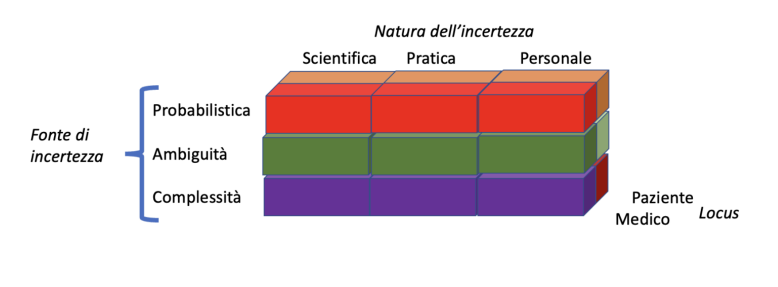
\includegraphics[width=0.9\columnwidth]{fonti-incertezza} 
    \caption{Natura dell'incertezza}
\end{figure}

Le situazioni cliniche possono essere rappresentate come costituite da un nucleo di rischio conosciuto, affrontabile con la conoscenza probabilistica, circondato da una nube di incertezza. La gestione dell'incertezza in medicina non dovrebbe limitarsi a una semplice ricognizione anamnestica, ma deve essere un aspetto chiave del metodo clinico, incorporato in tutti gli aspetti del processo decisionale dei professionisti sanitari. Questo è essenziale per attuare azioni appropriate.\\
\begin{figure}[!ht] 
    \centering 
    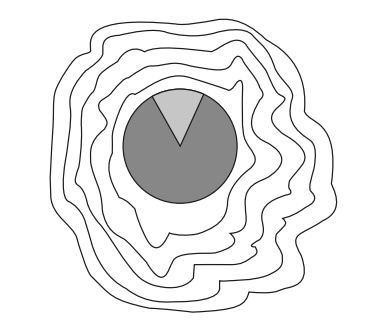
\includegraphics[width=0.9\columnwidth]{incertezza-situazioni-cliniche} 
    \caption{Illustrazione di come si presentano le situazioni cliniche}
\end{figure}


Nel processo decisionale clinico, l'incertezza influisce sulla probabilità che un evento si verifichi o meno. Riconoscere l'incertezza consente di comunicarla, prendere decisioni più consapevoli e praticare una medicina più prudente e meno onnipotente.
In base alle preferenze espresse dal paziente, possiamo costruire una rete protettiva (safety net) adottando una strategia di attesa. Prescriviamo un sintomatico e informiamo il paziente in modo strutturato sui sintomi di allarme (red flags) che potrebbero presentarsi, nonché sui tempi e le modalità per cercare aiuto medico se questi sintomi si manifestassero o se non ci fossero miglioramenti in un periodo prestabilito. Idealmente, queste informazioni dovrebbero essere fornite per iscritto, dopo un processo decisionale condiviso.\\

Esistono situazioni in cui la diagnosi è incerta e l'alternativa potrebbe essere una malattia grave a progressione rapida. In questi casi, si può utilizzare il tempo come un test, simile a un esame ematico o strumentale. L'aspetto comunicativo della strategia è cruciale. Il medico deve creare una buona relazione di fiducia e collaborazione con il paziente, affinché quest'ultimo possa comprendere chiaramente le istruzioni. Il paziente deve essere consapevole dell'incertezza diagnostica, dei segni e sintomi a cui prestare attenzione e del periodo di osservazione, nonché sapere come cercare aiuto.\\

È fondamentale anche l'aspetto organizzativo: il medico e il suo team devono avere accesso alle informazioni sulla decisione presa con il paziente in ogni momento, e deve esistere un sistema di ricezione delle chiamate che preveda una risposta immediata.\\

In generale, i risultati non sono sempre chiari, quindi gli autori invitano i medici alla prudenza, a utilizzare la rete protettiva e a insegnarla nel training della medicina generale, in attesa di maggiori risultati sull'efficacia di questa pratica. Tuttavia, lo strumento più potente per aiutare il medico a decidere nell'incertezza è la condivisione del processo decisionale con il paziente o con chi se ne prende cura.\\

In che modo il contributo del paziente può influire sul processo decisionale in medicina? Kon sostiene che la decisione condivisa esiste su un continuum con il modello paternalistico (guidato dal medico) a un'estremità e il modello informativo (guidato dal paziente) all'altra, mentre al centro c'è la \textit{decisione condivisa}\footcite{womak:decisione-condivisa-kon} in cui medico e paziente contribuiscono equamente, ciascuno al 50\%.\\


\begin{figure}[!ht] 
    \centering 
    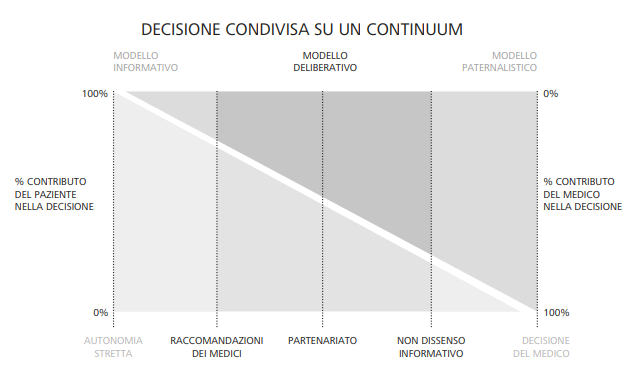
\includegraphics[width=0.9\columnwidth]{decisione-condivisa-kon} 
    \caption{Modello della decisione condivisa secondo Kon}
\end{figure}

Occorre considerare quale situazione clinica richiede un maggiore coinvolgimento del paziente. Questa è spesso una situazione di incertezza, contrapposta a una in cui esiste una chiara opzione migliore con un rapporto costi/benefici ben definito. In contesti incerti, le preferenze e i valori del paziente diventano cruciali poiché non ci sono rapporti chiari tra costi e benefici. Più è grande l'incertezza, più è necessario coinvolgere il paziente, valutando le sue conoscenze e capacità. Questo non significa solo considerare le preferenze, ma anche integrare il contributo del paziente nella decisione.\\

È importante distinguere la decisione condivisa dal semplice consenso informato. Quest'ultimo implica un flusso informativo unidirezionale dal medico al paziente, che è eticamente e legalmente obbligatorio ma non necessariamente parte di una decisione già presa dal medico. La vera decisione condivisa implica invece uno scambio di idee tra medico e paziente, una collaborazione che porta a una decisione comune. In questo processo, il paziente agisce come consulente, aiutando il medico a prendere una decisione, il che è molto diverso da un semplice processo informativo.


\section{Guida nell'analisi dell'incertezza secondo l'EFSA}
Il comitato scientifico dell'Autorità europea per la sicurezza alimentare (EFSA) ha sviluppato una guida dettagliata\footcite{womak:guida-analisi-incertezza} sull'analisi dell'incertezza nelle valutazioni scientifiche, con l'obiettivo di fornire una base solida per il processo decisionale in situazioni di incertezza.\\

Il comitato scientifico dell'EFSA è composto da eminenti scienziati di tutta Europa, ciascuno con una comprovata eccellenza scientifica e una vasta esperienza in varie discipline rilevanti per il mandato dell'EFSA. Tra le loro competenze si annoverano la valutazione dei rischi per la salute umana, l'epidemiologia, la microbiologia, la nutrizione umana, la chimica, la biologia e molte altre aree scientifiche. Questo gruppo multidisciplinare lavora per sviluppare metodologie armonizzate di valutazione del rischio e per garantire l'omogeneità dei pareri scientifici.\\

Le questioni affrontate dal comitato sono spesso di natura multidisciplinare, richiedendo approcci innovativi e integrati per la valutazione del rischio. Tra queste, vi sono l'armonizzazione dell'uso di ipotesi predefinite in assenza di dati reali.\\

Secondo tale comitato, l'analisi dell'incertezza nelle valutazioni scientifiche varia a seconda della natura della valutazione stessa. È essenziale identificare il tipo di valutazione in corso per poi seguire le linee guida specifiche.\\

Tipologie di Valutazione:
\begin{itemize}
    \item Valutazioni Standardizzate: Queste seguono procedure prestabilite e dettagliate, spesso utilizzate per prodotti regolamentati come le autorizzazioni di preimmissione sul mercato. Queste procedure richiedono dati da studi specifici e includono criteri e calcoli standardizzati.
    \item  Valutazioni Specifiche per il Caso in Esame: Necessarie quando non esistono procedure standardizzate. I valutatori devono sviluppare un piano di valutazione personalizzato, utilizzando elementi standardizzati dove possibile ma adottando approcci specifici per altre parti.
    \item  Elaborazione o Revisione di Documenti Orientativi: Coinvolge la creazione o l'aggiornamento di procedure standardizzate.
    \item  Valutazioni Urgenti: Richiedono completamento rapido con risorse limitate e implicano approcci semplificati.
    
\end{itemize}

In alcune aree dell'EFSA, una valutazione standardizzata può evidenziare la necessità di un'analisi più approfondita. In questi casi, si passa a una valutazione specifica per il caso, sostituendo elementi standardizzati con approcci su misura.
Le valutazioni possono essere quantitative (stima di una quantità) o qualitative (risposta verbale a una domanda). Anche se una valutazione è qualitativa, le conclusioni devono essere ben definite. L'incertezza può essere espressa quantitativamente tramite probabilità, pertanto, è raccomandato che i valutatori cerchino di quantificare l'incertezza anche quando utilizzano metodi qualitativi, poiché i metodi qualitativi hanno comunque un ruolo importante nell'analisi dell'incertezza.\\

\subsection{Analisi dell'incertezza per le valutazioni standardizzate}
Quando si analizza l'incertezza in una valutazione standardizzata, è cruciale distinguere tra incertezze standard e non standard. Prima di tutto, bisogna determinare se esistono incertezze non standard. Se non ci sono, basta riportare che la valutazione non presenta incertezze non standard. In caso contrario, bisogna valutare l'impatto di queste incertezze sul risultato della procedura standard. Se l'incertezza non standard è significativa, potrebbe essere necessario passare a una valutazione specifica per il caso in esame.\\

\subsection{Analisi dell'incertezza per valutazioni specifiche per il caso in esame}

Per le valutazioni specifiche per il caso, i valutatori devono seguire istruzioni pertinenti e, se necessario, consultare pareri scientifici di supporto. Dopo aver pianificato la valutazione e identificato le incertezze, bisogna decidere se suddividere l'analisi dell'incertezza in parti. Questa scelta dipende dalle domande e quantità rilevanti per la valutazione. \\
Valutare le incertezze collettivamente è il metodo più semplice, dove tutte le incertezze vengono valutate insieme nell'ambito della valutazione specifica.

Se l'analisi richiede risposte a domande sì/no, i valutatori possono esprimere le incertezze utilizzando probabilità e combinarle tramite calcoli. Questo richiede che ogni parte dell'analisi risponda a domande sì/no e che il ragionamento sia espresso in un modello logico formale. In alternativa, le incertezze possono essere valutate separatamente, sia qualitativamente che quantitativamente, e poi combinate secondo giudizio esperto. Anche se alcune parti vengono valutate qualitativamente, è consigliabile esprimere un giudizio di probabilità per la valutazione complessiva.\\

In caso di valutazioni scientifiche urgenti, i valutatori devono adottare un approccio rapido che si adatti ai tempi e alle risorse disponibili. Anche in situazioni di emergenza, l'analisi dell'incertezza è essenziale. Pertanto, si consiglia di valutare tutte le incertezze in un unico passaggio. Questo metodo, sebbene meno preciso rispetto ad altri, offre una base ragionevole per una consulenza preliminare, a condizione che l'incertezza aggiuntiva della valutazione semplificata sia chiaramente indicata nelle conclusioni.\\

Durante la creazione o la revisione di documenti di orientamento contenenti procedure standardizzate, è spesso necessario eseguire un'analisi dell'incertezza. Questa analisi verifica se la procedura proposta è sufficientemente prudenziale e se soddisfa gli obiettivi di gestione per quella specifica classe di prodotti o problemi. Una procedura ben calibrata può essere applicata ripetutamente senza dover valutare le incertezze standard ogni volta.\\

Se un'analisi dell'incertezza è richiesta per altri motivi durante lo sviluppo di un documento di orientamento, essa deve essere trattata come una valutazione specifica per il caso in esame. Quando una procedura viene utilizzata in più aree di lavoro dell'EFSA, la sua calibrazione e revisione devono essere svolte congiuntamente da tutti i soggetti coinvolti. Inoltre, se una procedura standardizzata fa parte di un protocollo internazionale, eventuali modifiche devono essere apportate in consultazione con i partner internazionali e la comunità scientifica.\\

\subsection{Individuazione delle incertezze}

\subsubsection{Incertezze standard e non standard}

Incertezze standard: Sono gestite da procedure standardizzate o da elementi standardizzati della valutazione. Ad esempio, nella valutazione del rischio chimico, un fattore di default pari a 100 può gestire le incertezze relative alla tossicità. In studi sperimentali, l'incertezza di misurazione è considerata standard se le linee guida sono state seguite senza deviazioni. Le incertezze standard non devono essere riconsiderate in ogni nuova valutazione che segue la procedura standard, poiché sono già state valutate durante la definizione della procedura stessa.\\

Incertezze non standard: Includono qualsiasi deviazione da una procedura standard o elementi non coperti dalla stessa. Ad esempio, studi che non seguono le linee guida standard o che presentano carenze nella reportistica, oppure l'uso di studi non standard o di "livello superiore". Queste incertezze devono essere valutate caso per caso, poiché non sono coperte dal margine di manovra delle incertezze standard.\\

Proporzione delle incertezze: In ogni tipo di valutazione possono esserci sia incertezze standard che non standard, ma in proporzioni variabili. Le valutazioni standardizzate tendono ad avere meno incertezze non standard, mentre altre valutazioni ne presentano di più.



\subsection{Procedure per l'individuazione delle incertezze} 

\textbf{Fonti di incertezza:} Ogni valutazione deve indicare le fonti di incertezza individuate, preferibilmente sotto forma di elenco o tabella, per trasparenza.

\textbf{Verifica sistematica:} I valutatori devono verificare sistematicamente le incertezze in ogni parte della valutazione, includendo sia gli input (dati, stime, evidenze) che i metodi utilizzati (metodi, calcoli, modelli statistici, ragionamento, giudizio esperto), per ridurre al minimo il rischio di tralasciare incertezze importanti. Nelle valutazioni standardizzate, devono essere individuate solo le incertezze non standard.

\textbf{Incertezze negli input:} Queste vengono individuate durante la valutazione delle evidenze dalla letteratura o dai database esistenti. Se sono disponibili approcci strutturati per la valutazione delle evidenze, dovrebbero essere utilizzati. Altrimenti, i valutatori possono usare la Tabella 1 come guida per individuare le incertezze negli input. Devono anche prestare attenzione a eventuali incertezze aggiuntive non elencate.

\textbf{Incertezze nei metodi}: Queste non sono generalmente gestite dagli schemi di valutazione delle evidenze esistenti. I valutatori dovrebbero utilizzare la colonna destra della Tabella 1 per individuare le incertezze nei metodi applicati alla valutazione. Anche qui, devono essere considerati eventuali tipi aggiuntivi di incertezza.

\textbf{Uso delle tabelle:} Le tabelle e gli elenchi devono facilitare l'individuazione delle incertezze, non la loro classificazione. I valutatori non dovrebbero impiegare troppo tempo a far corrispondere le incertezze alle tipologie elencate.

\textbf{Classificazione delle incertezze:} I valutatori devono determinare quali incertezze sono standard e quali non lo sono, poiché questo influenzerà come verranno gestite nei passaggi successivi dell'analisi dell'incertezza.

\begin{figure}[!ht] 
    \centering 
    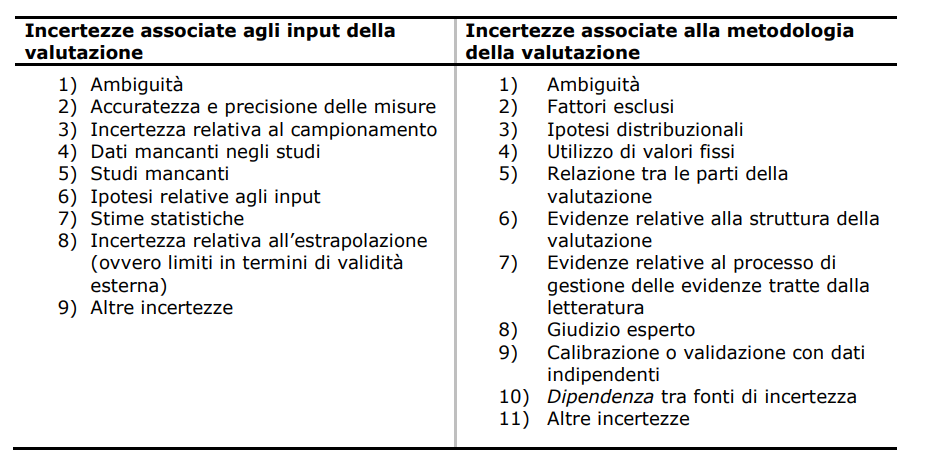
\includegraphics[width=0.9\columnwidth]{tipologia-incertezze} 
    \caption{Natura dell'incertezza}
\end{figure}

\subsubsection{Definizione delle priorità delle incertezze}

Definire le priorità delle fonti di incertezza è utile in diverse fasi della valutazione. All'inizio, aiuta a selezionare le incertezze più importanti per un'analisi approfondita. Durante la valutazione, individua le aree in cui cercare più dati o coinvolgere ulteriori esperti. Alla fine, identifica potenziali aree di ricerca futura. Le priorità dovrebbero basarsi sul contributo di ciascuna fonte di incertezza all'incertezza complessiva della valutazione, tenendo conto della dimensione dell'incertezza e della sua influenza sul risultato.
L'influenza delle diverse incertezze può essere valutata utilizzando giudizi esperti e scale ordinali. Si possono utilizzare metodi come le “tabelle d'incertezza” o l'approccio NUSAP.

Quando si usano modelli quantitativi, l'analisi di sensibilità può valutare l'influenza delle incertezze sugli input del modello. Le scelte riguardanti la struttura del modello possono essere verificate ripetendo la valutazione con alternative.

Per affrontare l'incertezza in modo efficace, è fondamentale che la valutazione sia suddivisa in parti principali, come esposizione e pericoli in una valutazione del rischio chimico, e in parti minori, come singoli parametri o studi. Questa suddivisione consente di eseguire l'analisi dell'incertezza a diversi livelli: valutare tutte le incertezze collettivamente, suddividerle in parti principali e combinarle successivamente, o suddividerle ulteriormente in parti più piccole e combinarle gradualmente. È essenziale combinare le parti dell'analisi per caratterizzare l'incertezza complessiva, definendo in anticipo come queste parti verranno integrate. Utilizzare un diagramma di modello concettuale può migliorare la trasparenza e il rigore del processo.\\

L'efficienza e l'affidabilità della valutazione dipendono dal livello di suddivisione scelto. Trattare separatamente le parti con incertezze rilevanti è generalmente più affidabile, mentre valutare tutte le incertezze collettivamente può essere più rapido ma meno preciso. Alcune incertezze minori possono essere considerate in una fase successiva della caratterizzazione complessiva, mentre quelle maggiori dovrebbero essere combinate tramite calcoli per garantire maggiore affidabilità. Quando si utilizzano modelli quantitativi, è utile quantificare l'incertezza per ciascun parametro e considerare anche le incertezze non quantificate, come quelle relative alla struttura del modello.\\

Per valutare correttamente l'incertezza, è essenziale che le domande e le quantità d'interesse siano chiaramente definite. Qualsiasi ambiguità aggiunge ulteriore incertezza e complica la valutazione. Se una domanda o quantità non è già ben definita, i valutatori devono provvedere a farlo per l'analisi dell'incertezza. Una quantità o domanda è ben definita se i valutatori possono concordare sulla risposta. Per ottenere ciò, si può specificare un esperimento, uno studio o una procedura che determinerebbe la risposta. Ad esempio, una misura ben definita per una quantità d'interesse dovrebbe includere specifiche di tempo, popolazione, luogo e condizioni. Allo stesso modo, la presenza o assenza di condizioni o meccanismi specifici deve essere dettagliata, così come i risultati di uno studio scientifico o un calcolo rilevante per la valutazione. Durante la formulazione delle domande, è importante identificare e sostituire termini ambigui o soggetti a giudizio di gestione del rischio con termini più chiari o numeri. Se i termini di riferimento sono aperti, è necessario che le conclusioni siano riferite a quantità ben definite o contengano affermazioni chiare e ben definite, necessarie per valutare ed esprimere l'incertezza associata.\\

L'espressione qualitativa dell'incertezza utilizza parole o categorie ordinali, senza quantificare le possibili risposte o probabilità. Questo metodo è utile in varie situazioni, come la definizione delle priorità delle incertezze e la descrizione di singole fonti di incertezza durante l'analisi. Le espressioni qualitative sono utili per definire le priorità, descrivere singole fonti di incertezza come passaggio preliminare per la quantificazione complessiva, comunicare i risultati usando una scala di probabilità approssimata con descrittori qualitativi, descrivere incertezze non incluse nella valutazione quantitativa e per la reportistica quando richiesto da decisori o normative.\\

Per descrivere singole fonti di incertezza, si raccomanda l'uso di scale ordinali per migliorare coerenza e trasparenza. Queste scale dovrebbero essere parte della pianificazione della valutazione e possono variare in formalità a seconda delle necessità. Le espressioni qualitative dovrebbero essere usate per elaborare un giudizio quantitativo sull'impatto combinato delle incertezze, basandosi su una logica chiara e non su calcoli arbitrari.\\

\subsection{Quantificare l'incertezza tramite probabilità}

Il Comitato scientifico raccomanda di esprimere quantitativamente l'impatto combinato delle incertezze. Le probabilità, specificate completamente o parzialmente, possono essere derivate da dati o giudizio esperto.\\

\textbf{Probabilità:} La probabilità varia da 0 a 1, espressa come percentuale da 0\% a 100\%. Per una domanda sì/no, 0\% significa che la risposta è sicuramente negativa, 100\% che è sicuramente positiva, e valori intermedi rappresentano vari gradi di certezza.\\

\textbf{Distribuzioni di probabilità:} L'incertezza relativa a una quantità non variabile può essere espressa tramite una distribuzione di probabilità, mostrando la probabilità relativa di diversi valori. Un'espressione parziale dell'incertezza può indicare la probabilità che un intervallo di valori includa il valore reale.\\

\textbf{Uso dei dati:} Quando disponibili, i dati dovrebbero essere utilizzati tramite analisi statistica, anche se il giudizio esperto interviene sempre, ad esempio nella scelta del modello  statistico. L'incertezza può essere quantificata direttamente o tramite calcoli dopo aver quantificato singole fonti di incertezza.\\

    \chapter{Sistemi di supporto alle decisioni}
\label{cap:sistemi-supporto-decisioni}

I Sistemi di Supporto alle Decisioni (DSS) sono strumenti informatici progettati per assistere gli utenti nel processo decisionale, utilizzando dati e modelli per risolvere problemi complessi e non strutturati. Questi sistemi combinano l'uso di dati, modelli analitici e strumenti di supporto interattivi per aiutare a prendere decisioni più informate. I DSS possono essere applicati in vari settori, tra cui il business, la sanità, la finanza e la gestione delle risorse umane.\\
Si suddividono in tre categorie principali:
\begin{itemize}
    \item DSS orientati ai dati: si concentrano sulla raccolta e l'analisi dei dati. Utilizzano database e data warehouse per memorizzare grandi quantità di dati e strumenti di data mining per estrarre informazioni utili.
    \item DSS orientati ai modelli: utilizzano modelli matematici e statistici per analizzare i dati e supportare il processo decisionale. Questi modelli possono includere modelli di ottimizzazione, simulazione, previsione e analisi delle serie temporali.
    \item DSS orientati alla conoscenza: incorporano conoscenze specifiche del dominio, regole e logiche di business per supportare decisioni complesse. Spesso utilizzano sistemi esperti e intelligenza artificiale per rappresentare e utilizzare la conoscenza.
\end{itemize}

I DSS hanno avuto una significativa evoluzione nel corso degli anni: originariamente erano semplici strumenti di analisi statistica utilizzati per supportare decisioni aziendali specifiche. Con l'avvento della tecnologia dell'informazione e delle comunicazioni sono diventati più complessi e potenti, integrando nuove tecnologie come il data warehousing, il data mining e, più recentemente, il machine learning e l'intelligenza artificiale (AI).\\
Negli ultimi anni, il machine learning è diventato una componente essenziale dei DSS moderni, infatti consente ai sistemi di apprendere dai dati e migliorare le loro prestazioni senza essere esplicitamente programmati. Questo è particolarmente utile nei casi in cui la capacità di analizzare grandi volumi di dati e identificare pattern nascosti può migliorare significativamente il processo decisionale.\\
È essenziale che i DSS moderni comunichino l'incertezza nei dati e nei risultati delle analisi. La trasparenza aiuta i decisori a comprendere i limiti delle previsioni e a prendere decisioni più informate. L'incertezza può derivare da vari fattori, tra cui la qualità dei dati, l'accuratezza dei modelli utilizzati e l'aleatorietà intrinseca dei fenomeni osservati \footcite{womak:role-decision-making}.\\
La comunicazione dell'incertezza è particolarmente importante in settori dove le decisioni hanno un impatto significativo sulla vita delle persone, come la sanità. Ad esempio, un DSS utilizzato per diagnosticare una malattia deve comunicare chiaramente l'incertezza associata alla diagnosi, in modo che i medici possano considerare tutte le possibili opzioni di trattamento.\\


\section{Machine learning in ambito medico }

Negli ultimi anni, l'IA ha conosciuto uno sviluppo significativo, rendendo possibile immaginare un futuro in cui diagnosi errate e trattamenti sintomatici saranno superati. La gestione e l'analisi delle enormi quantità di dati generate dalle immagini mediche e dai test diagnostici consentono all'IA di sviluppare applicazioni sofisticate, inaugurando un'era di medicina elettronica.\\
Nonostante alcuni algoritmi siano in grado di eguagliare e talvolta superare i clinici in varie attività, l'IA non è ancora integrata completamente nella pratica medica quotidiana.\\

Molti algoritmi di IA possono apprendere dai dati, sia che si tratti di immagini mediche (come le scansioni MRI) sia di dati numerici (come la pressione sanguigna). Dopo aver elaborato questi dati, gli algoritmi sono in grado di fornire risultati probabilistici o classificazioni, come identificare un campione di tessuto come canceroso o stimare la probabilità di un coagulo arterioso. Le prestazioni degli algoritmi vengono poi confrontate con quelle dei medici per determinare se la diagnosi dell'IA è accurata e clinicamente rilevante.\\

Un esempio significativo di IA in ambito medico è l'algoritmo DLAD (Rilevamento Automatico basato su Apprendimento Profondo)\footcite{site:intelligenza-artificiale-medicina}, sviluppato presso l'Università Nazionale di Seoul. Questo algoritmo analizza le radiografie del torace per rilevare crescite cellulari anomale, come i tumori. Nei test comparativi, DLAD ha dimostrato di superare 17 su 18 medici nella capacità di rilevamento delle anomalie.\\
Un altro esempio significativo di algoritmo IA nel settore medico è stato sviluppato nell'autunno del 2018 dai ricercatori di Google AI Healthcare\footcite{site:intelligenza-artificiale-medicina}. Questo algoritmo, denominato LYNA (Assistente dei Linfonodi), è stato progettato per identificare i tumori metastatici del cancro al seno dalle biopsie dei linfonodi. LYNA rappresenta un progresso significativo poiché è in grado di individuare aree sospette nei campioni di biopsia, una capacità che va oltre la percezione visiva umana. Nei test condotti su due diversi database, LYNA ha dimostrato un'accuratezza del 99\% nel classificare i campioni come cancerosi o non cancerosi. Inoltre, ha ridotto della metà il tempo medio di revisione delle diapositive quando utilizzato dai medici come supporto alla loro analisi tradizionale.\\
Altri algoritmi basati su immagini hanno mostrato abilità simili nel migliorare l'accuratezza diagnostica dei medici. \\
Esempi come DLAD e LYNA dimostrano come gli algoritmi possano supportare i medici nella classificazione di campioni patologici, evidenziando caratteristiche delle immagini che necessitano di un'analisi più approfondita.\\

Recentemente è stato condotto un nuovo studio\footcite{womak:machine-learning-in-orthopedics} che esplora l'applicazione delle tecniche di machine learning (ML) in ambito ortopedico; il suo focus è esaminare articoli pubblicati negli ultimi vent'anni e farne una revisione.\\
In questo studio il machine learning è definito come lo studio di come gli algoritmi possono "imparare" relazioni complesse dai dati empirici, producendo modelli matematici che collegano numerose variabili a una variabile target di interesse. In medicina, questo significa poter prevedere, data una serie di immagini radiologiche, risultati di laboratorio o dati estratti da registri elettronici, etichette diagnostiche, livelli di risultato, valori di esami o opzioni di trattamento per aiutare i medici a prendere decisioni più accurate ed efficienti.\\
La revisione della letteratura è stata condotta eseguendo una ricerca sui database Medline e Scopus, includendo articoli che utilizzano tecniche di ML per il sistema muscoloscheletrico umano. Sono stati selezionati sei settori anatomici principali: colonna vertebrale, anca, ginocchio, caviglia, mano e piede, oltre a una procedura generale, l'artroplastica. Sono stati selezionati 70 articoli per una revisione approfondita del loro contenuto e codifica.\\
Gli articoli sono stati divisi in due categorie principali: tecniche di ML convenzionali e deep learning.
Tecniche di ML convenzionali:
\begin{itemize}
\item Decision Trees e Random Forests: Queste tecniche sono state utilizzate per classificare i soggetti con osteoartrite e per fornire interpretabilità clinica dei risultati.
\item Nearest Neighbors (NN): Utilizzate per varie applicazioni, tra cui la segmentazione delle immagini.
\item Regressione Lineare e Altre Tecniche Simili: Impiegate per modellare relazioni lineari tra variabili.
\item Support Vector Machines (SVM): Ampiamente usate per la classificazione e il rilevamento delle caratteristiche.
\item K-means Clustering e Altre Tecniche Simili: Utilizzate per raggruppare i dati in base a caratteristiche simili.
\item Altre Tecniche Discriminative: Come gradient boosting machines e LDA.
\item Tecniche Generative: Come i modelli probabilistici, utilizzati per prevedere la progressione della scoliosi.
\end{itemize}
Gli autori hanno concluso che, sebbene il ML abbia dimostrato risultati promettenti in vari campi ortopedici, è necessaria una valutazione rigorosa e una validazione in contesti reali prima che possa essere ampiamente adottato nella pratica clinica. Attualmente, l'adozione del ML in ortopedia è ancora in una fase preliminare, con necessità di ulteriori studi e ricerche per consolidarne l'applicabilità e l'efficacia.


% \subsection{Deep Learning}
% Il deep learning, una sottocategoria del ML che utilizza reti neurali profonde, è particolarmente efficace per la gestione di grandi volumi di dati, come immagini mediche e dati sensoristici. Questo metodo è stato applicato a diverse aree dell'ortopedia, dimostrando un'elevata precisione in compiti come la segmentazione delle immagini e la classificazione delle patologie.\\
% I risultati sono stati presentati anche visivamente, mostrando l'uso predominante delle tecniche di deep learning e SVM nei dati di imaging medico. Le analisi bibliometriche indicano un crescente interesse per l'applicazione del ML in ortopedia negli ultimi anni, con una tendenza verso l'uso di tecniche più avanzate e la collaborazione tra diversi gruppi di ricerca.\\

\section{Visualizzazioni vaghe}
\label{sec:visualizzazione-vaghe}
Le visualizzazioni vaghe sono un concetto importante in data science che aiuta a gestire l'incertezza e la variabilità nei dati. Quando si tratta di analisi dei dati, spesso ci troviamo a dover affrontare informazioni che contengono errori, rumore o incertezze intrinseche. Le visualizzazioni vaghe sono progettate per rappresentare queste incertezze in modo che gli utenti possano avere una comprensione più completa e affidabile delle informazioni presentate.\\
Uno dei metodi più comuni utilizzati nelle visualizzazioni vaghe è l'impiego degli intervalli di confidenza: questi intervalli indicano la gamma di valori entro cui si prevede che un parametro si trovi con una certa probabilità. Ad esempio, in un grafico a barre, possiamo vedere delle linee verticali che rappresentano l'intervallo di confidenza per ciascuna barra, fornendo così un'indicazione visiva dell'incertezza associata a ciascun dato.\\
Nei grafici a linee, le bande di incertezza sono spesso utilizzate per mostrare la variabilità intorno a una linea di tendenza. Queste bande, che possono essere ombreggiate, offrono una rappresentazione visiva chiara dell'incertezza, aiutando a comprendere meglio quanto ci si può fidare di una previsione o di una tendenza osservata. Anche le mappe di calore (heatmaps), sono strumenti efficaci in questo contesto, poiché possono rappresentare dati spaziali o temporali con variazioni di colore o intensità per indicare incertezze.\\
I grafici di tipo violin plot e box plot sono altre tecniche utili, poiché permettono di visualizzare la distribuzione dei dati insieme alle indicazioni di variabilità e densità.\\
In sostanza la visualizzazione vaga si propone di rappresentare dei risultati non in formato numerico o simbolico, ma attraverso immagini pittoriche in cui prevale un'incertezza visiva. Questo tipo di rappresentazione visiva è legata a tre fattori principali: vaghezza, indistintitezza e sfocatura. \\

Attualmente, nelle scienze dure, come la matematica, la logica e le scienze naturali (biologia, chimica, fisica), l'incertezza viene rappresentata in termini di probabilità, punteggi di confidenza o percentuali. In questo approccio non è sempre chiaro se l'incertezza venga realmente compresa dai medici, con conseguente rischio di sopravvalutare le informazioni, un fenomeno noto come bias della quantificazione\footcite{womak:vague-visualizations-quantification-bias}.\\
Secondo lo studio "Vague Visualizations to Reduce quantification bias in shared medical decision making", dalle immagini è possibile trarre valori numerici in modo "immediato" attraverso diverse modalità, come la posizione su scale graduate, segmenti su un piano cartesiano, angoli o sfumature di colore.\\
Lo scopo delle visualizzazioni vaghe è quindi sfruttare il gut feeling degli utenti, ovvero lasciare che sia la loro percezione a guidarli piuttosto che la razionalità.\\

L'incertezza può essere rappresentata con varie tecniche e modalità. Non è stata ancora definita la “forma” migliore da utilizzare, ma quello che sembra ormai certo è che colore, tonalità, saturazione del colore, forma e la trasparenza siano i mezzi più efficaci. In questo studio comparativo si è evidenziato che la sfocatura, la posizione e la trasparenza favoriscono la percezione e l'intuizione da parte del fruitore finale, mentre la saturazione risulta meno utile. Relativamente alla tecnica da utilizzare, come ad esempio i glifi di linea, alcuni ricercatori hanno evidenziato che la tecnica stessa dipende anche dalla capacità di "traduzione" o decodifica dell'utente finale.\\

In questo studio si è voluto valutare l'efficacia rappresentativa di tre effetti visivi, precisamente: la sfocatura, la trasparenza e il rumore, nel comunicare una probabilità di rischio. Gli autori intendono per efficacia rappresentativa la rappresentazione, e quindi la soluzione grafica, che permette valutazioni coerenti, senza indurre l'utente a sovrastimare o a sottostimare il valore della probabilità. È evidente che le VV non devono ostacolare la comprensione o fuorviare i medici nelle loro valutazioni e scelte diagnostiche e terapeutiche.\\ 
Lo studio si è posto due domande:
\begin{itemize}
    \item la VV ostacola o favorisce la stima delle probabilità?
    \item In caso di risposta affermativa, c'è qualche effetto tra quelli utilizzati che è più efficace o meno
    fuorviante degli altri?
\end{itemize}
Per testare le domande è stato creato un software web based che accetta qualsiasi immagine raster (formata da pixel) e una percentuale di probabilità come input, e restituisce in output la medesima immagine influenzata però dagli effetti visivi precedentemente specificati. Il 100\% di probabilità coincide con l'immagine originale, quindi purezza al 100 per cento; il valore 0\% corrisponde alla massima distorsione e viene rappresentata la massima incertezza.
Nello studio sono state create 6 visualizzazioni con le seguenti percentuali: 10\%, 25\%, 40\%, 60\%, 75\% e 90\%; queste percentuali corrispondono a diversi \gls{quartili}.

\begin{figure}[!ht] 
    \centering 
    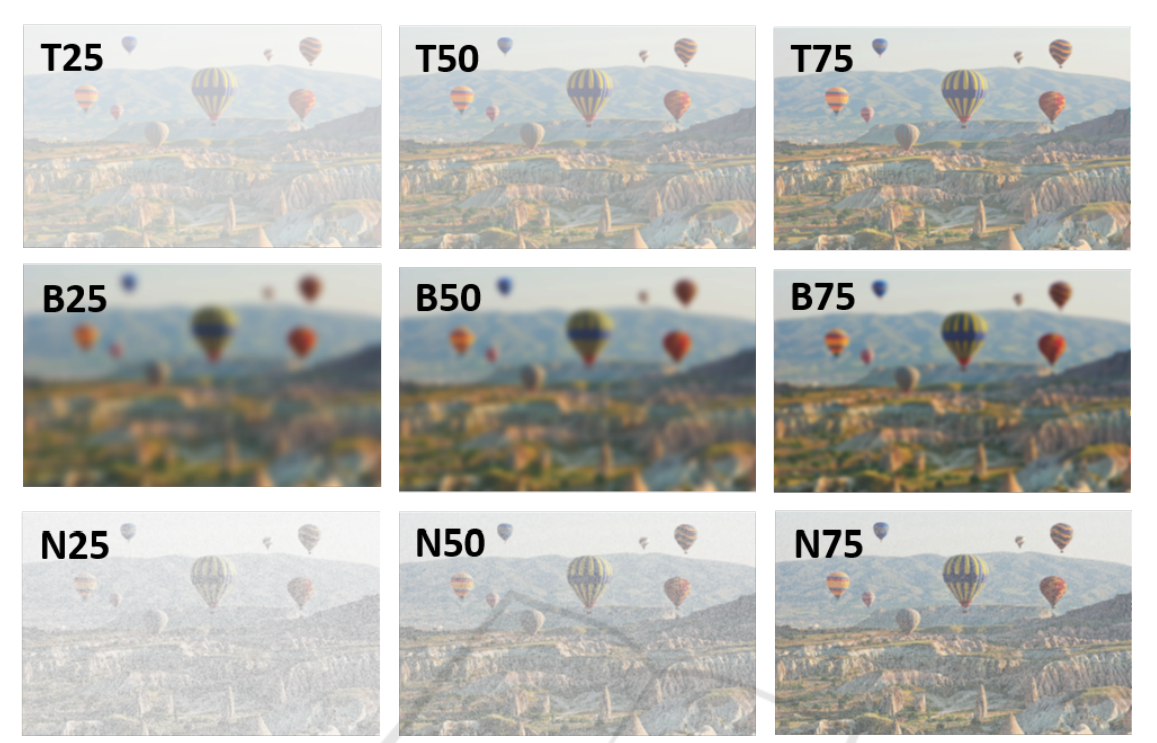
\includegraphics[width=0.9\columnwidth]{transparency-blur-noise} 
    \caption{Effetti applicati all'immagine per rendere il rischio del 25\%, 50\% e 75\%. T, B e N sono, rispettivamente, l'effetto della trasparenza, sfocatura e rumore}
\end{figure}

È stato strutturato un questionario online proposto poi a un certo numero di studenti universitari e conoscenti. I partecipanti avevano come compito quello di associare due delle 6 VV (2VV scelte casualmente per ogni effetto visivo) in due compiti di difficoltà crescente. Per tutti e due i compiti, è stato somministrato un set di riferimento a tre VV che indicavano un valore del 0\%, 50\% e 100\%, rispettivamente.\\
In questo questionario il primo compito riguardava l'accuratezza visiva (RA), il secondo compito l'accuratezza assoluta.
Nel presentare le visualizzazioni su cui si basava il questionario si ipotizzavano due possibili fonti di bias che avrebbero potuto influenzare l' analisi:
\begin{itemize}
\item l'ordine delle domande (bias di ordine);
\item il valore della percentuale mostrata (ovvero, bias di campionamento).
\end{itemize}

Per ridurre il primo tipo di bias, il questionario online è stato implementato in modo che la presentazione dei 3 effetti diversi ai partecipanti fosse in ordine casuale.\\
Le VV sono risultate utili nel comunicare probabilità sotto e sopra il 50\%, con una tendenza a sovrastimare i valori bassi e a sottostimare quelli alti. Non sono emerse differenze significative tra sfocatura, trasparenza e rumore, eccetto la trasparenza, più efficace al 40\%.\\
In particolare le visualizzazioni vaghe sono uno strumento valido per comunicare valori intermedi, mentre è stata registrata una regressione alla media quando vengono mostrati valori estremi.\\
Infine, non è stato individuato un metodo migliore di altri. Gli studiosi contano di effettuare altri esperimenti in ambienti controllati e reali per verificare se le decisioni prese dai medici sono diverse quando la previsione del rischio è rappresentata con quantità evidenti, o mediante una visualizzazione vaga. Si conta anche di misurare la soddisfazione dei medici.\\

Un altro studio interessante che utilizza le visualizzazoini vaghe è lo studio "Comparative Assessment of Two Data Visualizations to Communicate Medical Test Results Online"\footcite{womak:comparative-assesment}, dove si prendono in esame test diagnostici basati su biomarcatori, cioè indicatori di una specifica condizione, nella fattispecie l'infezione da SARS-CoV-2, causa di COVID-19.\\
Ogni test diagnostico, sia esso basato su imaging, carica virale o presenza di antigeni, è associato a un certo margine di errore, ma razionalmente tendiamo a considerare l'esito del test solo in termini di sì/no, evitando di valutare la probabilità di avere o non avere una specifica condizione. Utilizzando gli strumenti di supporto decisionale basati su ML, l'elemento probabilistico può essere reso visibile e quindi esplicitato, ad esempio riportando i punteggi di probabilità o rappresentandoli in un qualche modo: in questo studio i ricercatori ritengono che questo possa aiutare gli utenti ad interpretare al meglio l'output della macchina. In pratica l'incertezza intrinseca di questi modelli può costituire un plus nel processo decisionale, ad esempio per scegliere se sottoporsi ad un ulteriore esame o per prediligere una terapia.\\
Tale studio ha quindi lo scopo di scegliere la migliore visualizzazione dei dati da presentare agli utenti relativamente ad un test ematologico per rilevare le infezioni da COVID-19, mediante il Conteggio Ematologico Completo, utilizzando un modello di ML. Questo modello è stato convalidato nella letteratura di riferimento e poi incorporato in uno strumento basato sul Web.\\
Sono state confrontate due visualizzazioni progettate secondo i principi delle visualizzazioni vaghe: le stime incerte sono rappresentate evitando volutamente l'utilizzo dei simboli, cioè numeri e rappresentazioni metriche, come estensioni della lunghezza e angoli. Secondo le caratteristiche delle visualizzazioni vaghe, le quantità probabilistiche sono presentate come indizi visivi, i quali sono difficili da interpretare in termini razionali, cioè sono difficili da associare a valori numerici. Si utilizzano specificamente tonalità di colore o gradienti di saturazione e luminosità. Questa modalità è voluta e mira a comunicare ai lettori un senso di incertezza e vaghezza per far sì che i lettori comprendano effettivamente le stime visualizzate, come rischi, probabilità, dispersione. È evidente che le visualizzazioni vaghe richiedono una attenzione aggiuntiva.\\

Le due visualizzazioni citate sono state ideate durante due sessioni di progettazione in cui sono stati coinvolti sia gli autori di questo articolo sia i clinici che hanno sviluppato il modello statistico. I clinici sono stati adeguatamente edotti circa le caratteristiche delle visualizzazioni vaghe e sono stati invitati a co-progettare due visualizzazioni: una visualizzazione destinata a colleghi esperti nell'interpretare i test di laboratorio, e una più semplice che potesse essere più familiare ai pazienti testati.\\
Le visualizzazioni risultanti si basavano su metafore diverse: la prima visualizzazione si basava sul comune \gls{test-del-tornasole} e sulla metafora della bolla livello; la seconda visualizzazione dei dati adottava la metafora del bastoncino di test, utilizzata, ad esempio, nei test di gravidanza, e quindi familiare al pubblico in generale.
Lo studio è stato concepito per capire:\\
\begin{enumerate}
    \item se la metafora del bastoncino di test fosse adeguata in caso di una risposta sensibile e delicata
    come quella relativa alla positività al COVID-19, o, come osservato in alcuni studi, finisse per
    confondere troppo spesso le persone comuni
    \item se una visualizzazione dei dati più tecnica, quella progettata per gli operatori sanitari, potesse
    essere comprensibile anche al pubblico comune.
\end{enumerate}
Nella visualizzazione a bolla livello, il risultato del test è presentato attraverso la posizione di una bolla circolare all'interno di una barra a tre colori (simile al tornasole). Si valuta quindi la sua maggiore o minore vicinanza a uno degli estremi della barra per indicare una condizione COVID-19-positiva o negativa (rispettivamente all'estremo rosso più a sinistra e all'estremo blu più a destra). I risultati incerti, cioè quelli a bassa affidabilità, sono caratterizzati da una sostanziale equidistanza della bolla dagli estremi, corrispondente ad un posizionamento nella zona grigia centrale della barra tornasole. L'incertezza è anche resa evidente dalla dimensione della bolla: più grande è la bolla, maggiore è l'intervallo di confidenza della stima della probabilità.\\

\begin{figure}[!ht] 
    \centering 
    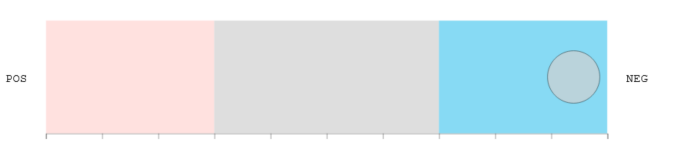
\includegraphics[width=0.9\columnwidth]{metafora-bolla} 
    \caption{Natura dell'incertezza}
\end{figure}

\begin{figure}[!ht] 
    \centering 
    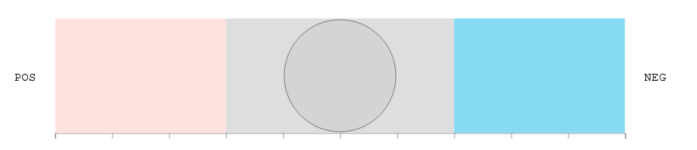
\includegraphics[width=0.9\columnwidth]{metafora-bolla-2} 
    \caption{Natura dell'incertezza}
\end{figure}

La visualizzazione del bastoncino di test fornisce le medesime informazioni visualizzate tramite la bolla livello, ma attraverso affordance (in senso generale, favorire l'utilizzo) e segnali visivi diversi.\\
Nel dettaglio si vedono due fasce rosse: una per indicare l'affidabilità della risposta e indicata con una C maiuscola ("controllo"), e una che indica il risultato del test, indicata con un segno più singolo (+). In pratica questa visualizzazione restituisce l'output del modello in termini di opacità della barra: più trasparenti (e meno visibili) sono la fascia + e la fascia C, minore è la probabilità che il test sia associato a una condizione positiva e che il test sia affidabile. Un test quasi certamente negativo è quindi reso da un bastoncino in cui è chiaramente visibile solo la barra C,mentre un test non valido è rappresentato da un bastoncino in cui nessuna fascia rossa è  visibile.
    \chapter{User Experience }
\label{cap:user-experience}

\subsection{Il progetto in partenza}
Inizialmente, l'applicazione era composta da due sole pagine: una per il wizard in cui l'utente compilava il form di dettaglio del paziente, e una seconda per la visualizzazione dei risultati, dove i grafici erano disposti in una griglia che occupava tutto lo spazio disponibile. Una delle principali carenze del POC iniziale era la mancanza di contesto nei grafici. Questo rendeva difficile la comprensione per utenti senza un background in data science, poiché non potevano interpretare correttamente i dati senza una spiegazione preliminare.\\

Un ulteriore problema riscontrato riguardava la lunghezza del wizard, che inizialmente consisteva di quattro step. Successivamente, un passo è stato eliminato e accorpato al primo per migliorare l'usabilità.

\subsection{Modifiche apportate}

Nella transizione da POC a software completo, il numero di pagine è aumentato: una per il wizard, una per i risultati, una per la valutazione dell'utente circa la piattaforma, e una per il tutorial. Il tutorial è stato posizionato nell'header per garantire un facile accesso da parte dell'utente in qualsiasi momento. Inoltre, il wizard è stato semplificato, eliminando uno step.\\

La pagina dei risultati ha subito le modifiche più significative. È stato inserito un tabbar che permette all'utente di cambiare le visualizzazioni. L'ordine del tabbar è stato progettato in modo tale che l'utente possa vedere prima le singole visualizzazioni e poi tutte insieme in una vista complessiva. Quando si clicca sul tab "All graphs", appare un modale bloccante, che l'utente non può chiudere senza prima compilare il form contenuto al suo interno. Questo form deve essere compilato solo una volta ed è cruciale per raccogliere dati sull'utilità percepita dal medico quando visualizza i vari grafici.\\
È possibile accedere a un altro form tramite il pulsante "Evaluate platform" posizionato in linea con il tabbar. Questo form raccoglie feedback sull'utilità percepita del software nel suo complesso.\\

\begin{figure}[!ht] 
    \centering 
    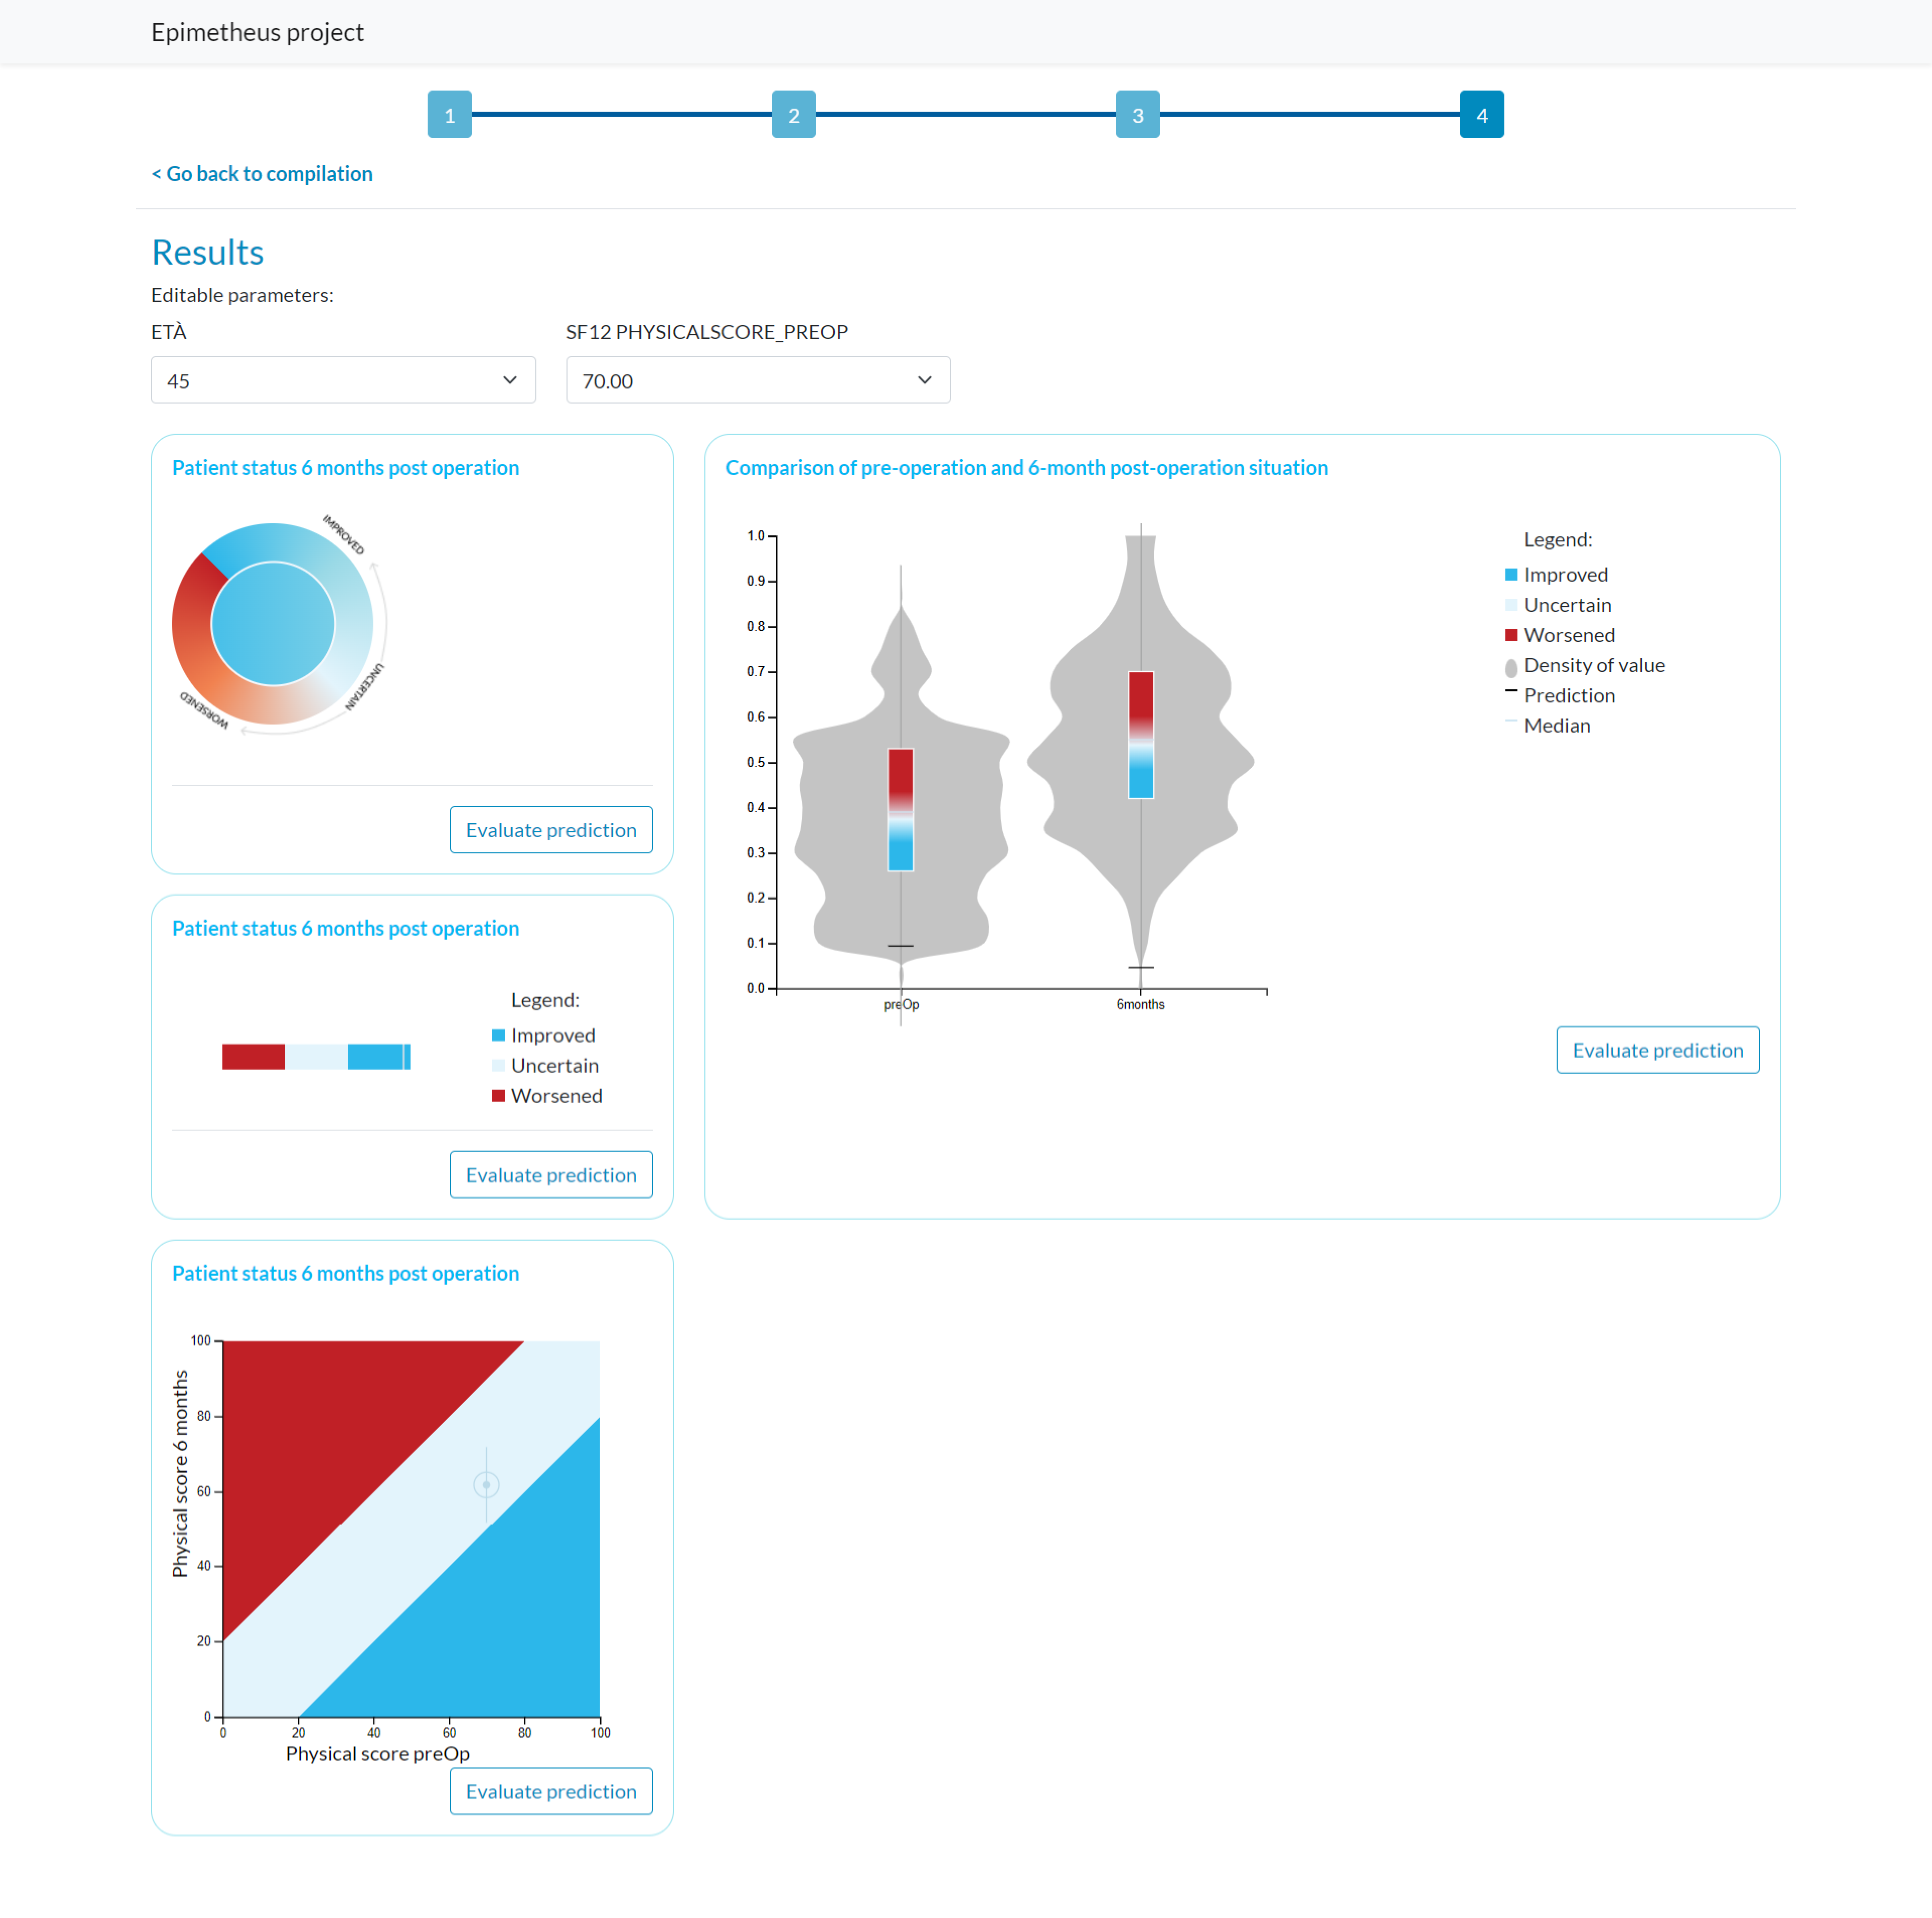
\includegraphics[width=0.5\columnwidth]{epi-start-results} 
    \caption{Pagina di risultati pre-modifiche}
\end{figure}

\begin{figure}[!ht] 
    \centering 
    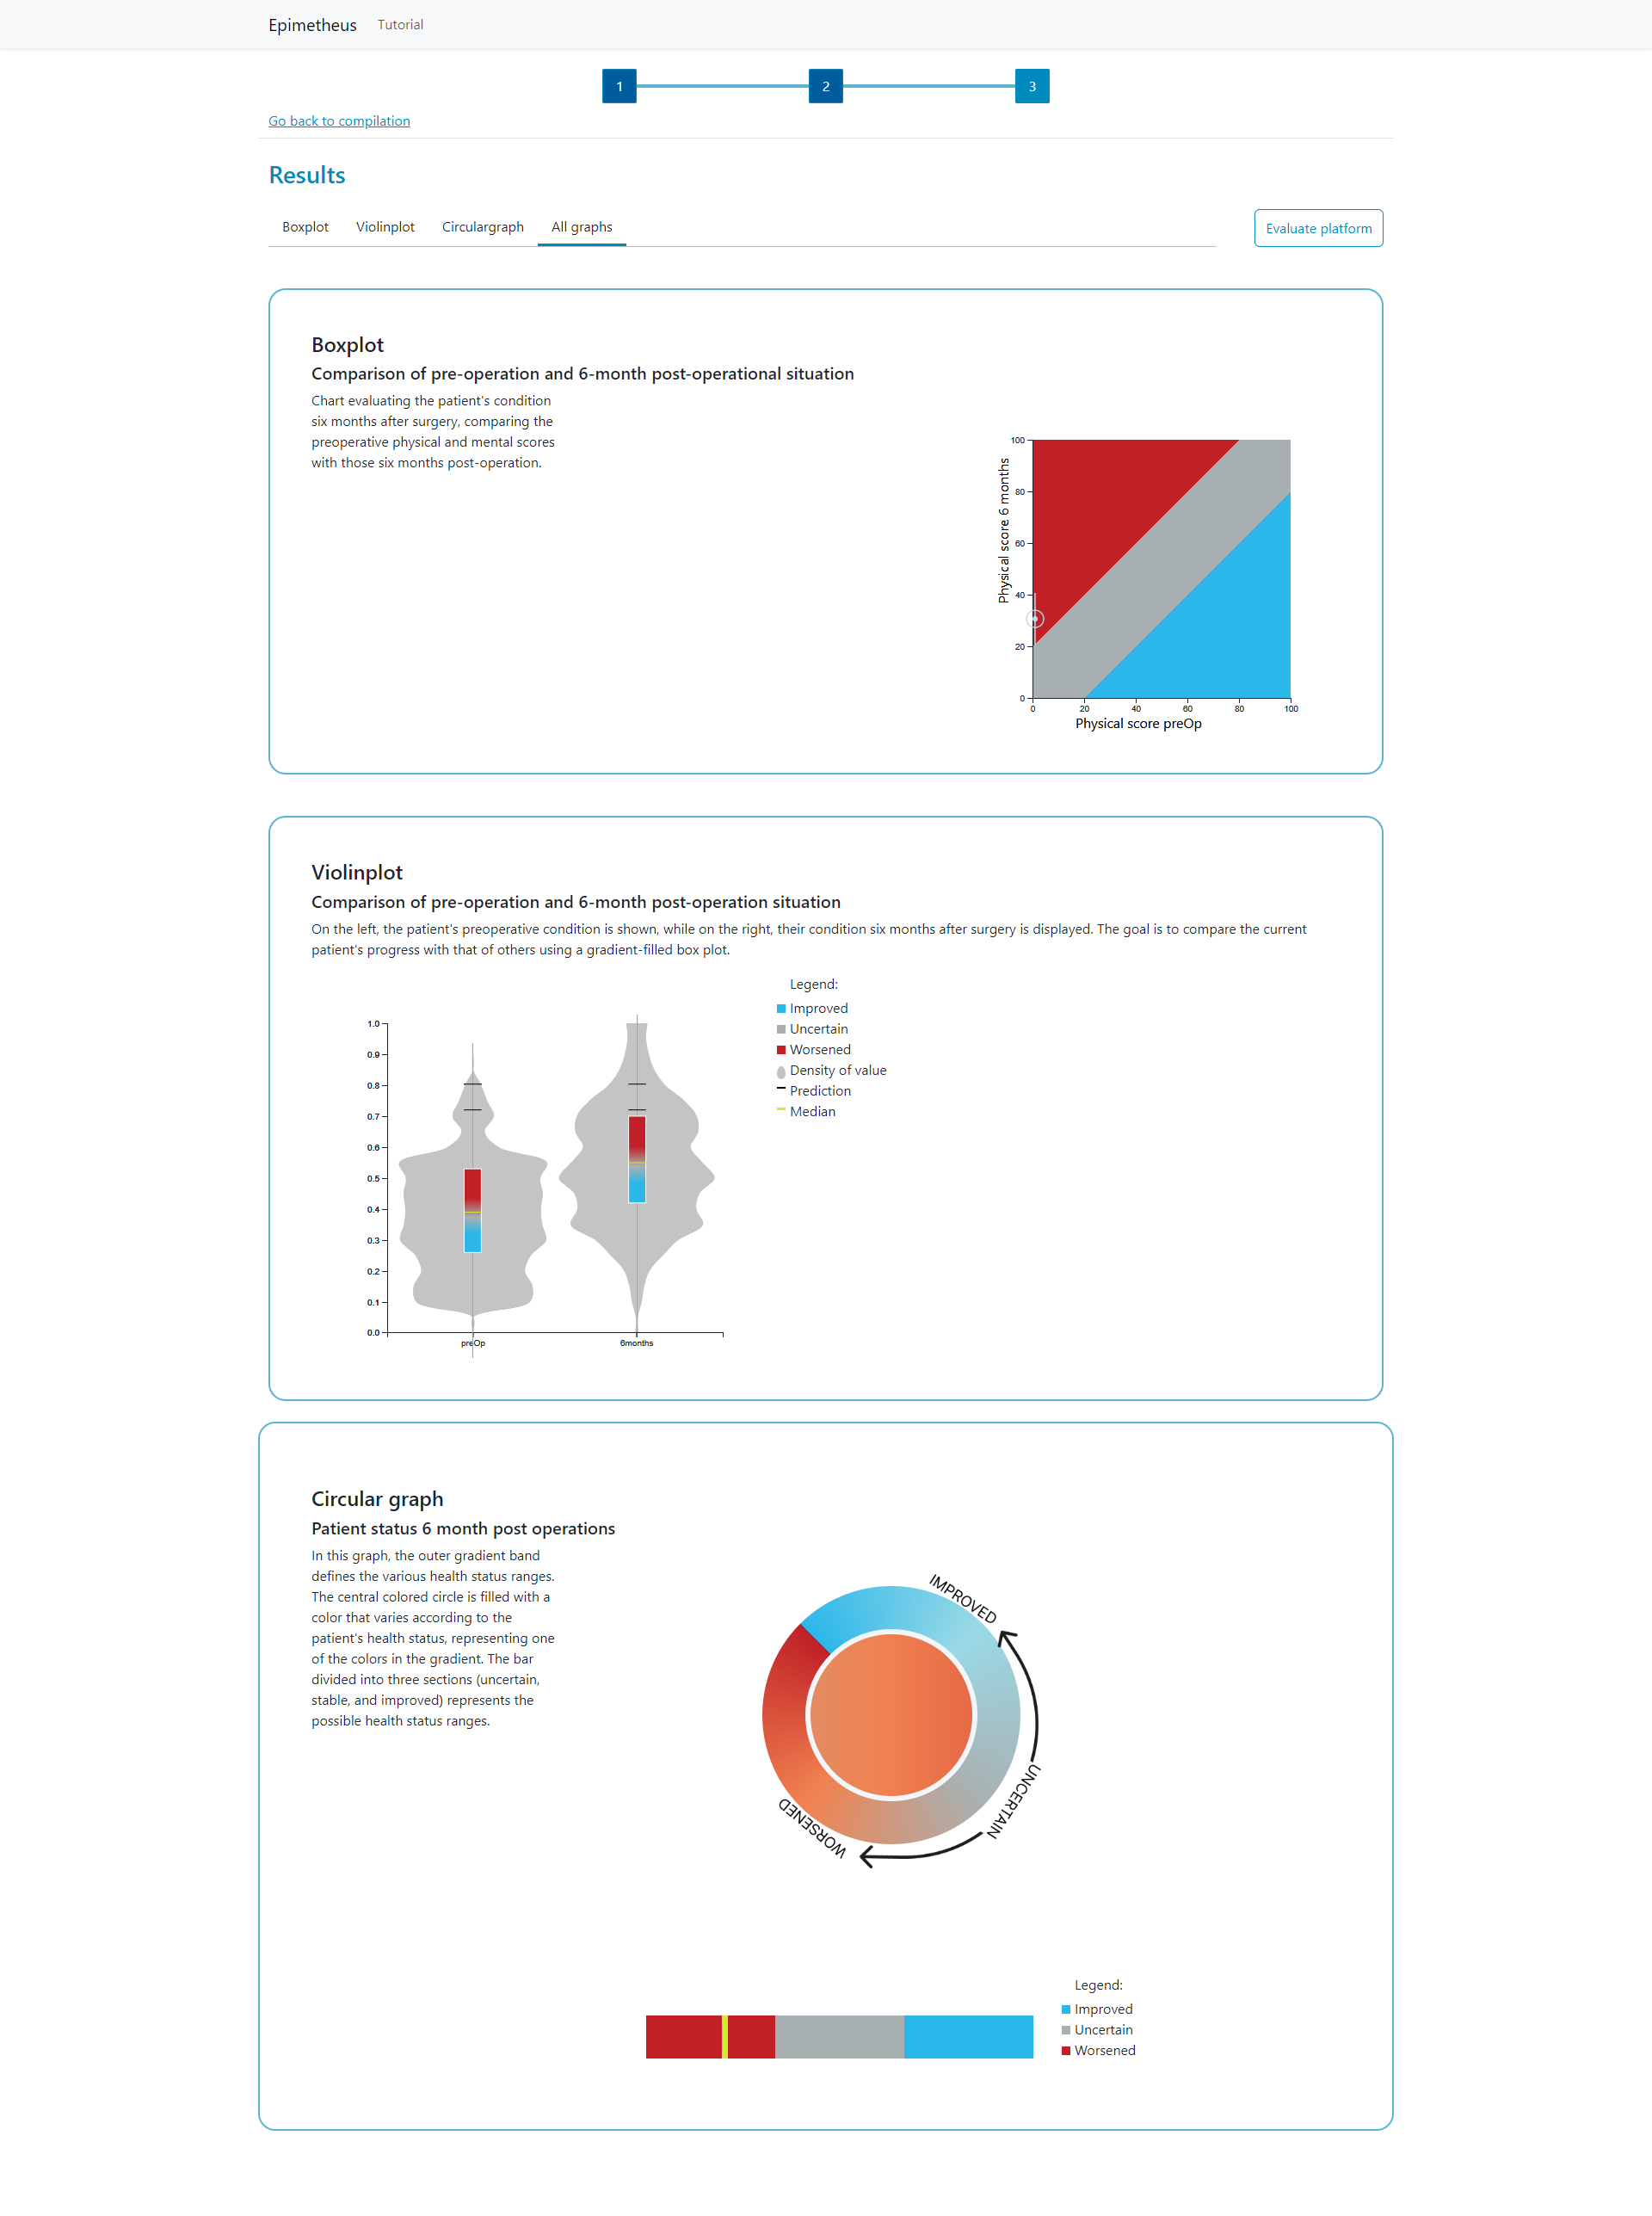
\includegraphics[width=0.5\columnwidth]{epi-all-graphs} 
    \caption{Pagina di risultati post-modifiche}
\end{figure}

I grafici sono interattivi, permettendo all'utente di modificare parametri specifici, come il valore del peso, con conseguente ricalcolo del grafico. Sono state inoltre apportate modifiche ai colori dei grafici. Inizialmente, il colore dell'incertezza era il celeste, ma poiché l'azzurro è il colore primario del brand identity del prodotto, ho deciso di sostituirlo con il grigio. Il grigio, per definizione, si presta meglio a rappresentare il dubbio e l'incertezza. A supporto della mia tesi, test condotti su un campione demograficamente variegato hanno confermato che il grigio è percepito come colore "incerto".\\

\section{Test}
Sono stati condotti due tipi di test, un questionario volto a fornire dati quantitativi e qualitativi, e dei think aloud volti a fornire dati qualitativi. \\

\subsection{Questionario}
Il questionario è stato somministrato a 42 utenti di diversa età ed estrazione sociale. Tra le prime domande che sono state poste vi è la domanda se sono soliti ad consultare grafici o infografiche nell'ambito del loro lavoro o per interesse personale; circa il 42\% di loro ha risposto di si, il 52\% di loro ha risposto di no. Successivamente si è indagato se gli utenti si ritengono esperti in grafici, il 42\% di loro ha risposto "abbastanza", il 36\% di loro ha risposto "non molto". La maggior parte degli utenti sceglie come fonte da cui visualizzare grafici siti web e libri di testo.\\
Successivamente il questionario si è articolato su domande relative ai colori e ai grafici. Qui ho indagato come gli utenti percepiscono l'incertezza, quindi ho posto una prima domanda volta a capire se la scelta del grigio invece dell'azzurro comunicasse meglio il concetto di incertezza. 

\begin{figure}[!ht] 
    \centering 
    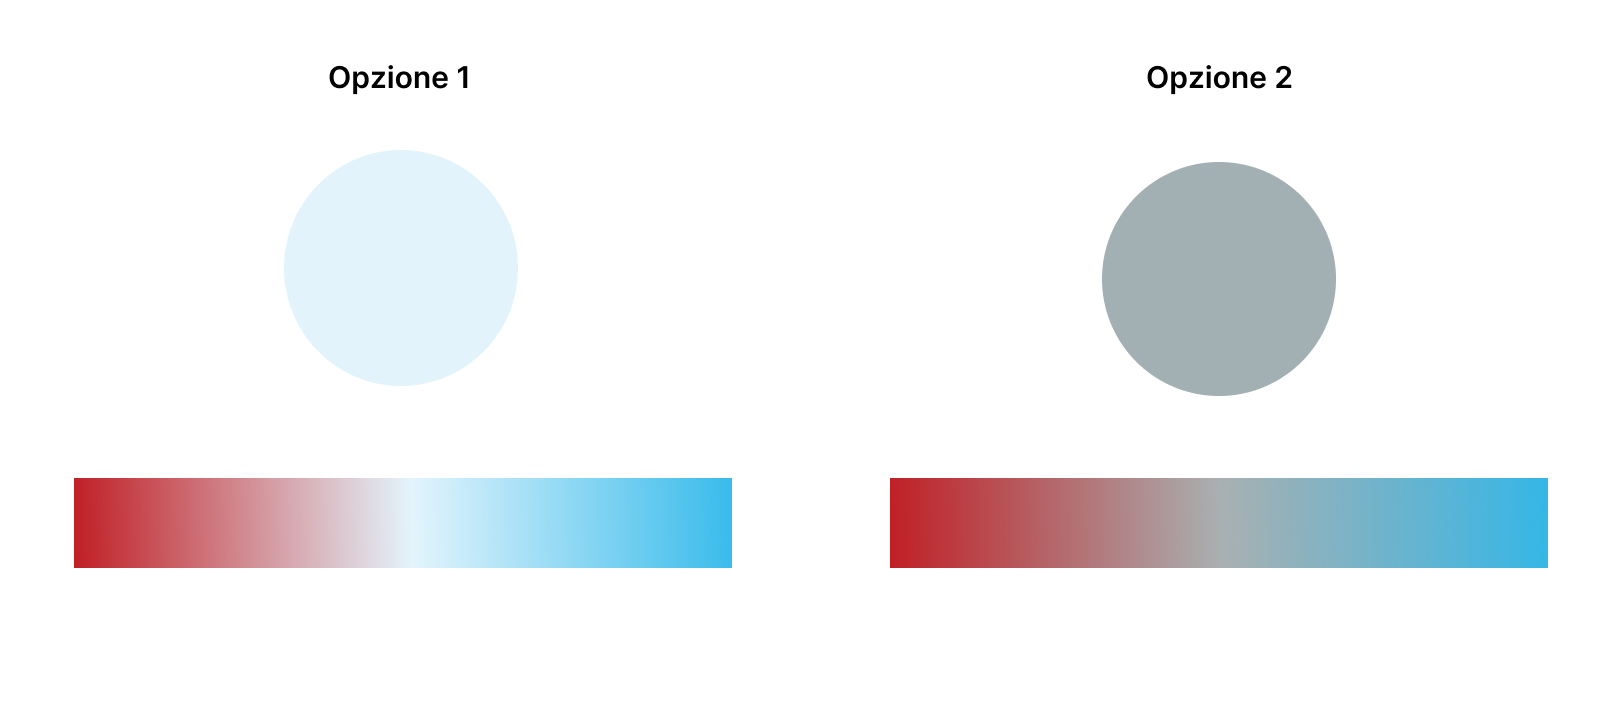
\includegraphics[width=0.7\columnwidth]{gradienti-a-confronto} 
    \caption{I due gradienti messi a confronto, focus posto sull'area centrale che rappresenta l'incertezza}
\end{figure}

% \begin{wrapfigure}{r}{0.3\textwidth}
%     \centering
%     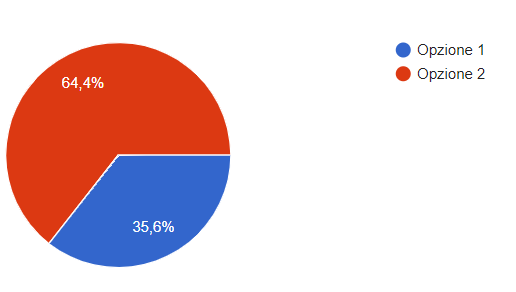
\includegraphics[width=0.4\textwidth]{domanda-colore-incertezza}
%     \caption{I due gradienti messi a confronto}
% \end{wrapfigure}

\begin{figure}[!ht] 
    \centering 
    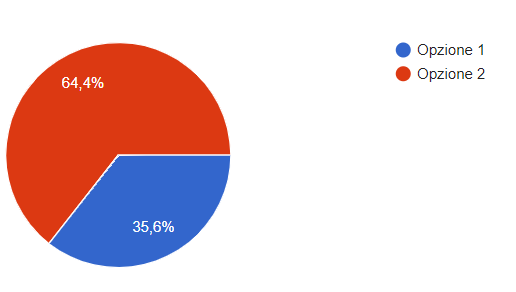
\includegraphics[width=0.3\textwidth]{domanda-colore-incertezza}
    \caption{Risposta degli utenti}
\end{figure}

Ne è emerso che l'intuizione era corretta, infatti il 64\% ha affermato di percepire maggiore incertezza utilizzando il colore grigio invece che azzurro. 

In un'altra sezione ho indagato sulla percezione dell'incertezza nell'ambito del grafico "Circulargraph". In particolare si voleva capire se effettivamente gli utenti percepissero correttamente lo stato di salute che si voleva comunicare. Per condurre questo test ho realizzato alcune copie del grafico, il colore del cerchio centrale è stato prelevato a partire da vari punti del gradiente esterno. Successivamente all'interno del questionario ho disposto i grafici in maniera casuale, in modo tale che l'utente non avesse un bias di ordine. \\

\begin{figure}[!ht] 
    \centering 
    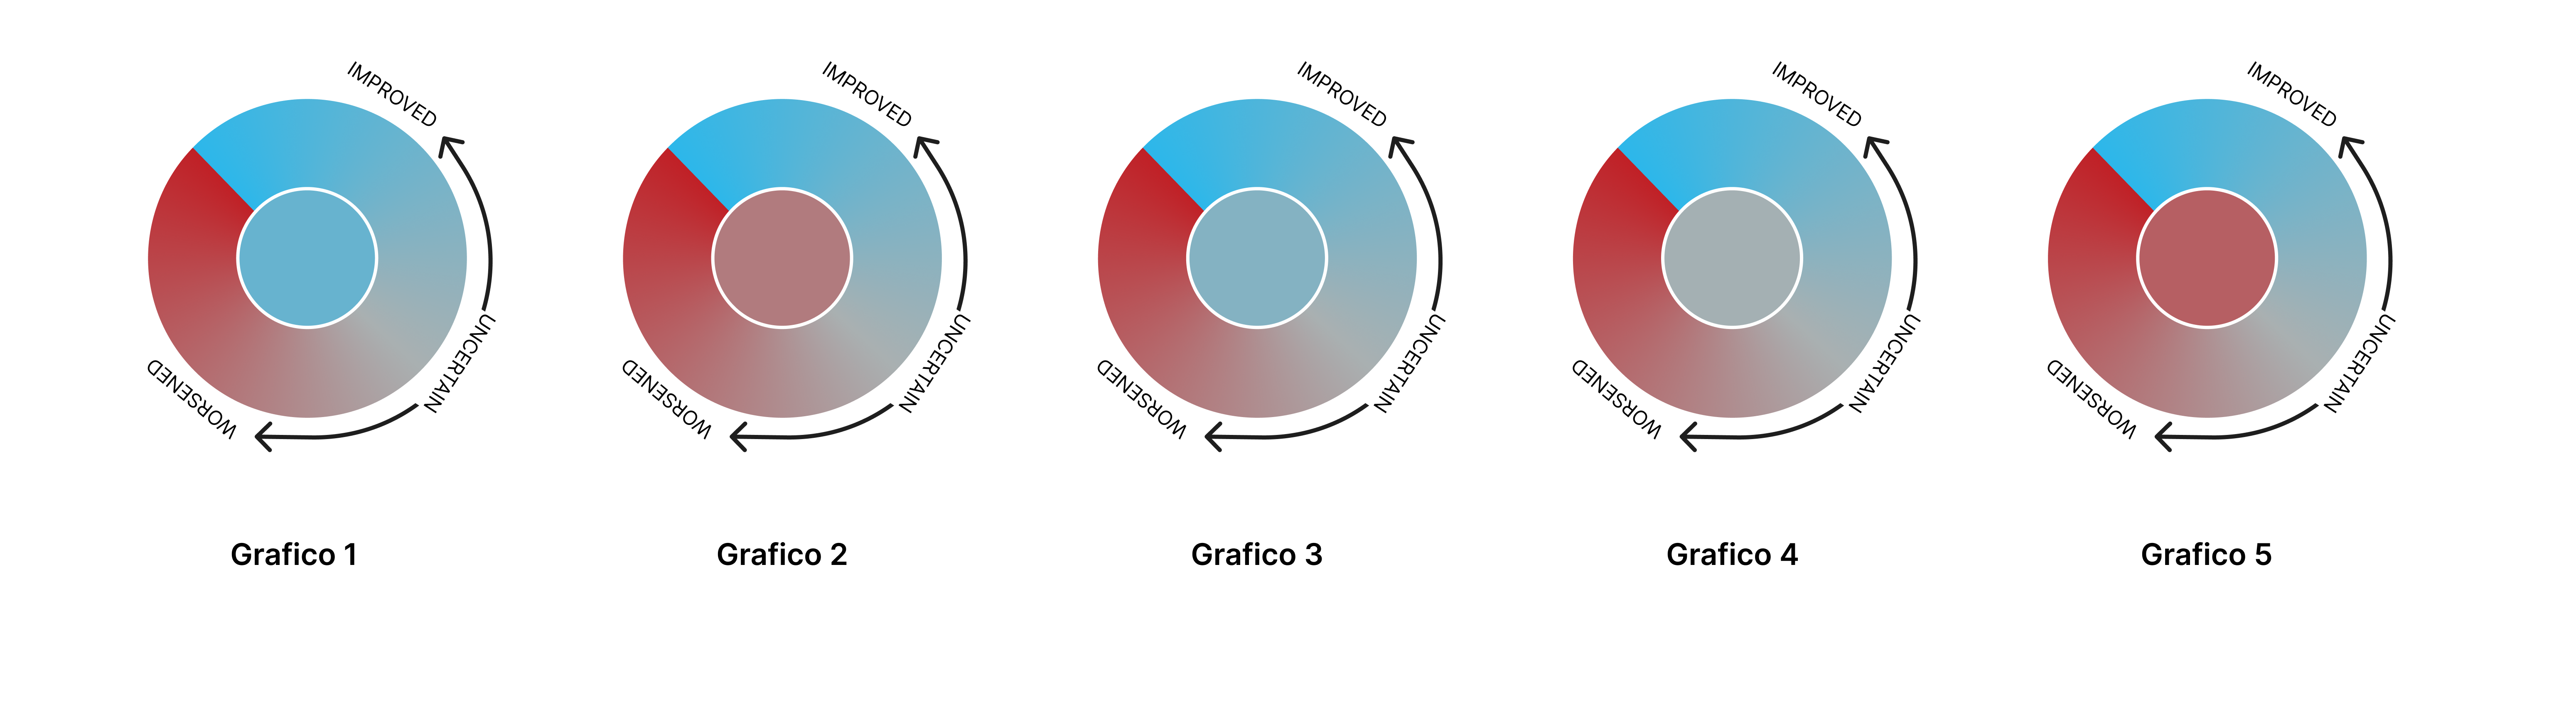
\includegraphics[width=0.9\textwidth]{domande-circulargraph}
    \caption{I circulargraph sottoposti a quesito}
\end{figure}

I risultati sono stati i seguenti:
\begin{itemize}
    \item Nel grafico 1 il 45,2\% degli intervistati ritiene che il paziente avrà un discreto miglioramento; il 42,9\% ritiene che avrà un netto miglioramento;
    \item Nel grafico 2 il 76,2\% degli intervistati ritiene che il paziente avrà un discreto peggioramento;
    \item Nel grafico 3 il 63,3\% degli intervistati ritiene che il paziente avrà un discreto miglioramento;
    \item Nel grafico 4 l'83,3\% degli intervistati ritiene che il paziente avrà un esito incerto, non si può dire se migliorerà o peggiorerà;
    \item Nel grafico 5 il 47,6\% degli intervistati ritiene che il paziente avrà un netto peggioramento, mentre il 38,1\% ritiene che avrà un discreto peggioramento.
\end{itemize}
Le conclusioni che si possono trarre da questi dati sono che il colore centrale effettivamente comunica correttamente quale sarà lo stato di salute del paziente. Inserire una legenda che permetta di capire quale è il colore del miglioramento e quale è il colore del peggioramento fornisce ulteriori indicazioni all'utente per orientarsi. \\

Ultima domanda ha riguardato un test A/B, in particolare si è messo a paragone le due pagine di risultati pre (opzione 1) e post (opzione 2) modifiche, e si è chiesto agli utenti quali delle due opzioni preferissero e perchè. Il 92,5\% dei partecipanti ha affermato di preferire la nuova interfaccia di risultati; i motivi riportati sono stati vari, tra i principali si può citare come motivazione una maggiore pulizia dell'interfaccia, l'interfaccia è meno stancante alla vista, è più ordinata, il commento che accompagna i grafici ne favorisce la comprensione. La parola più frequente è stata "lineare". \\
Tra questi vi è un commento in particolare che vale la pena citare: 
\begin{quote}
    \textit{Se l'intento è quello di avere un quadro chiaro e completo del paziente la prima opzione è la migliore perché sono visualizzate più informazioni in poco spazio, dando un quadro generale dello stato di salute; si perde però il dettaglio o delle note che potrebbero risultare comunque interessanti in caso di pazienti/operazioni particolari che invece nella seconda opzione potrebbero essere più facili da individuare.}
\end{quote}
Questo commento mi ha fatto pensare che in futuro si potrebbe aggiungere un bottone che cambi il layout dell'interfaccia, in modo tale da avere una visualizzazione raggruppata oppure una visualizzazione a lista.
    \chapter{Sviluppo software}
\label{cap:sviluppo-software}

\section{Design dei Sistemi}
Nell'ambito dello sviluppo software ho implementato quello che si chiama \textit{Design di Sistemi}, il quale si è reso essenziale per comprendere e gestire le interazioni tra le varie componenti del sistema. Questo approccio mi ha permesso di assicurare che tutte le parti dell'interfaccia lavorassero insieme in modo coerente ed efficiente.\\
Ho analizzato l'architettura del sistema, identificando tutte le componenti principali e le loro interazioni. Questo includeva il backend, il frontend, e le API utilizzate per la comunicazione tra le diverse parti del sistema.\\
L'obiettivo era garantire che il frontend fosse perfettamente allineato con le funzionalità offerte dal backend, facendo da filtro iniziale per avere una buona tolleranza all'errore dell'utente ed evitare il rischio di navigare in pagine di errore di difficile gestione o comprensione per l'utente 
inesperto. \\

Per implementare il Design dei Sistemi, ho utilizzato un approccio modulare, suddividendo l'interfaccia in componenti riutilizzabili. Ogni componente è stato progettato per essere indipendente e facilmente integrabile con gli altri, seguendo i principi della progettazione a strati. Ho separato il frontend (React) dal backend (Flask), garantendo che ciascuno potesse essere sviluppato, testato e aggiornato indipendentemente. Questa separazione ha facilitato non solo la manutenzione del software, ma in futuro permetterà l'implementazione di nuove funzionalità, garantendo un'evoluzione più rapida del prodotto.\\


\section{Il progetto in partenza}
Il software nasceva come POC, era un monolite unico dove backend e frontend risiedevano nella stessa directory.\\
Il backend, scritto in python, si occupava di:
\begin{itemize}
    \item esporre un endpoint per il frontend 
    \item realizzare calcoli di machine learning per generare le visualizzazioni 
\end{itemize}

Il frontend invece era composto da due file html, uno per il form e uno per la visualizzazione dei grafici, due file javascript, uno per la validazione del form e uno per la realizzazione dei grafici, e un file css che dava lo stile a tutto il sito. 

\section{Analisi e motivazioni}

Dopo una prima analisi del software e un confronto con gli stakeholder ho proposto di operare una divisione più netta di frontend e backend avvalendomi dell'ausilio di un framework per il frontend. Attraverso questa scelta si è seguito il principio di progettazione architetturale noto come \textit{Architettura a Strati} o \textit{Architettura a Livelli} (Layered Architecture).

Nell'architettura a strati, l'applicazione è suddivisa in diversi strati logici o livelli, ognuno dei quali ha una responsabilità specifica. Nel caso di Epimetheus:
\begin{enumerate}
\item Backend (Strato logico):
    \begin{itemize}
        \item  Responsabilità: Gestisce la logica di presentazione, in particolare la generazione delle risposte API per il frontend.
        \item  Tecnologie utilizzate: Flask, Python, API REST.
    \end{itemize}
\item Frontend (Strato di Presentazione):
 \begin{itemize}
    \item Responsabilità: Interagisce con l'utente e invia richieste API al backend per ottenere e visualizzare i dati.
    \item Tecnologie utilizzate: React, JavaScript, HTML, CSS.
 \end{itemize}
\item Strato di Persistenza: gestisce il salvataggio e il recupero dei dati.
    \begin{itemize}
        \item Gestione dei dati nel frontend: quando l'utente inserisce i dati, questi vengono salvati nel local storage del browser, un tipo di storage lato client che permette di mantenere i dati localmente e persistenti anche dopo la chiusura del browser.
        \item Gestione dei dati nel backend: i dati raccolti dai form di valutazione del prodotto vengono salvati in un file CSV locale. Questo approccio, noto come persistenza su file locale, permette di conservare i dati di valutazione per eventuali analisi future senza dover implementare subito un database più complesso
    \end{itemize}

\end{enumerate}

\noindent Questa separazione ha permesso di ottenere la divisione delle responsabilità, facilitando la manutenzione e l'aggiornamento dei singoli componenti senza influenzare gli altri.\\
La modularità introdotta permette inoltre di scalare l'applicazione con maggiore facilità, ad esempio nel caso in futuro si volesse applicare moduli di registrazione e login, quindi avere cura della sicurezza, oppure ampliare il numero di grafici da mostrare all'utente. \\
Il mio focus era principalmente la possibilità di permette in futuro di ampliare il software operando un limitato numero di modifiche, quindi era importante portare fin da ora il frontend ad una discreta maturità.

\section{Sviluppi}
Gli sviluppi sono proseguiti in parallelo tra me e i colleghi che ho coordinato. Io mi sono occupata principalmente del frontend, sono partita dall'interfaccia del wizard mentre ho indirizzato e supportato i colleghi nella realizzazione di endpoint, correzione del backend e creazione del salvataggio dei questionari compilati dagli utenti sulla piattaforma.\\
Dapprima sono stati realizzati endpoint separati per la validazione e il submit del form relativo ai dati del paziente. Successivamente, su mia indicazione, le logiche sono state accorpate in un unico endpoint che rispondesse con la visualizzazione oppure elencasse i campi non validi. La validazione è stata implementata sia lato frontend che lato backend per garantire maggiore robustezza.\\

\subsection{React}
Il frontend è stato sviluppato in React, le principali librerie usate sono state:
\begin{itemize}
    \item \textbf{Bootstrap}: per lo stile e alcuni componenti preconfezionati.
    \item \textbf{Axios}: per le chiamate API.
    \item \textbf{Toastify}: per mostrare notifiche (toast) in fase di validazione del form del paziente.
    \item \textbf{D3.js}: per la creazione dei grafici a partire dai dati pervenuti dal backend
\end{itemize}

\noindent Queste librerie sono state installate attraverso il package manager npm, facilitando la gestione delle dipendenze del progetto. Il vantaggio di npm è l'accesso a migliaia di pacchetti open source, rendendo più semplice l'aggiornamento e la gestione delle librerie utilizzate, e la messa a disposizione di script di build per effettuare il build e deploy del progetto. 

\subsection{Flask}
Flask è un microframework per Python, è stato scelto per la sua semplicità e flessibilità in quanto consente di costruire applicazioni web leggere e modulari.
Ho operato modifiche anche al backend, in particolare nella risposta inviata al frontend per calcolare le visualizzazioni. In origine, tra i campi modificabili vi era l'età, ma a seguito di analisi si è concluso che non era una dimensione di interesse per il medico-utente, pertanto è stata sostituita con il peso.\\ 
Ho inoltre predisposto la POST degli endpoint che ricevono i form di valutazione dell'utente, in modo tale che il collega maggiormente incentrato sul backend potesse successivamente sviluppare le feature per il salvataggio a CSV del form compilato.\\
La struttura del backend è così composta: 
\begin{itemize}
    \item \textbf{flaskapp.py}: è il punto d'ingresso principale per lanciare il progetto e contiene le rotte e le logiche di gestione delle richieste.
    \item \textbf{utils.py}: è il file dove sono presenti tutte le funzioni che si occupano di realizzare le visualizzazioni da inviare al frontend.
\end{itemize}

\subsection{Validazione}
Il software opera una doppia validazione:
\begin{itemize} 
    \item una lato frontend quando l'utente compila i campi, in modo tale da avere subito feedback se qualcosa non è corretto; questa viene fatta tramite chiamata a funzioni di validazioni implementate inizialmente dalla collega e successivamente evolute da me affinchè funzionassero in ambiente React. 
    \item una lato backend, il quale controlla il form pervenuto e verifica se sia tutto conforme.
\end{itemize}

\noindent Se lato frontend non dovessero esserci segnalazioni di errori, ma al contrario il backend dovesse rispondere con un errore, questo viene notificato al frontend e l'utente può vedere a video una pagina di errore con la descrizione di cosa è andato storto. Nel caso in cui il backend dovesse rispondere errore 500 l'utente vedrà una pagina di errore con descrizione generica. 

\subsection{La struttura}
Lato frontend le pagine principali sono le seguenti:\\ 
\begin{itemize}
    \item \textbf{Wizard:} è presente il wizard iniziale dove l'utente compila i dati del paziente; si compone di 2 step:  il primo è la scelta della zona da operare, il secondo è l'effettivo inserimento manuale dei dati del paziente.
    \item \textbf{Results:} è la pagina di risultati dove l'utente visualizza i grafici e interagisce con gli stessi.
    \item \textbf{Evaluation:} è la pagina di valutazione dell'applicativo, dove è presente un form che l'utente può compilare per darci il suo feedback. 
    \item \textbf{Tutorial:} è una pagina accessibile dall' header che descrive l'applicativo e funge appunto da tutorial per l'utente. 
\end{itemize}
All'interno di queste pagine è possibile trovare diversi componenti volti a suddividere ulteriormente la complessità delle pagine e delle logiche.\\ 

Lato frontend mi sono avvalsa inoltre di alcuni pattern, tra i quali lo \textit{State Management Patterns} utilizzando il \textit{global context}, ovvero un contesto globale che permette di condividere informazioni tra i diversi componenti senza dover sottostare alla relazione parent-child. All'interno del global context possiamo trovare la gestione degli step, gran parte del form iniziale compilato dall'utente in quanto molte informazioni sono necessarie in più pagine e componenti, i dati fetchati in quanto servono alla pagina Results per calcolare le visualizzazioni. Il global context si occupa anche di controllare anche se parte di questi dati sono già presenti nel local storage del browser, quindi di inizializzare le rispettive strutture dati.\\

Il fetch delle API relative al submit del wizard avviene tramite custom hooks; questa scelta è stata fatta perchè in base a quale operazione l'utente sceglie di esplorare, vengono chiamati endpoint differenti. Il custom hooks ha permesso quindi di articolare queste logiche più strutturate su un file a parte dividendo opportunamente le responsabilità dei vari componenti. Utilizzare custom hooks assieme al global context ha permesso inoltre di semplificare la gestione delle informazioni condivise all'interno dell'applicativo.\\

La costruzione del wizard compilato dall'utente avviene in maniera dinamica, questo vuol dire che in base alla prima preferenza espressa dall'utente (spine o hip/knee) i campi da compilare cambieranno. Questa scelta è stata fatta per più motivi: inizialmente le operazioni da esplorare erano tre, ovvero hip, knee, spine; in base alla scelta dell'utente i campi del form erano effettivamente diversi, ed era ridondante utilizzare componenti react differenti in base al form necessario. Per implementare questa feature mi sono avvalsa dell'uso di un JSON di dati, dove viene inserita la lista di campi che devono comparire, le loro caratteristiche, ovvero con che nome devono essere inviati a backend e che tipo sono (number, text, select, radio), e quale sarà la funzione che si occuperà dalla validazione. Questa implementazione permette di poter ampliare il prodotto aggiungendo altre preferenze in modo facile e rapido, limitando quindi le modifiche da apportare ad due soli file per il frontend (il JSON con la lista dei campi e la lista di funzioni di validazione). 

\begin{figure}[!ht] 
    \centering 
    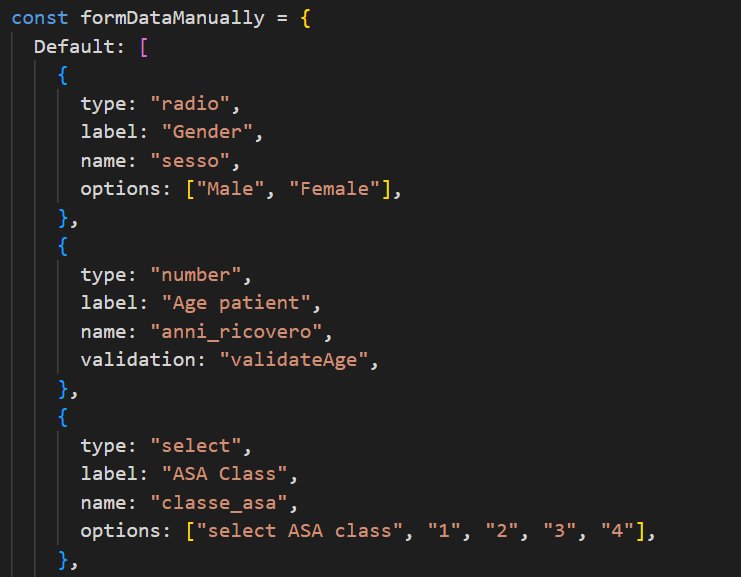
\includegraphics[width=0.9\columnwidth]{dynamic-form-example} 
    \caption{Natura dell'incertezza}
\end{figure}

    \chapter{Metodologia}
\label{cap:metodologia}

% \intro{Breve introduzione al capitolo}\\

\section{Metodologia agile e EventStorming}
\label{sec:metodologia-agile}

Gli sviluppi si sono svolti seguendo la metodologia agile\footcite{site:agile-manifesto}: sono state schedulate due riunioni mensili allo scopo di tenersi aggiornati sugli sviluppi in corso, in assenza di riunioni c'è comunque stato scambio di messaggi per mantenere presente e continua la comunicazione.\\
Il principio di fondo che si è seguito è quello dello sviluppo iterativo, ovvero tenendo presente l'obiettivo finale del software si è proceduto per step implementando prima soluzioni più semplici ed immediate e poi si è proceduto nell'evoluzione di alcune funzionalità per implementare soluzioni più performanti e scalabili. \\

Le comunicazioni all'interno del team si sono basate su riunioni online, di persona e condivisione di materiale informativo per accordarci sul lavoro da svolgere.\\
Il materiale usato è stato condivisione di documenti drive e di file Figma, nello specifico parte integrante dell'attività di comunicazione è stata l'uso dell' EventStorming\footcite{womak:event-storming}.\\
L'EventStorming è una tecnica collaborativa utilizzata principalmente per esplorare e modellare processi complessi e sistemi software attraverso la narrazione di eventi che accadono all'interno di un sistema. È stata sviluppata da Alberto Brandolini nel 2013 ed è particolarmente utile nel contesto del Domain-Driven Design (DDD). L'obiettivo principale di EventStorming è di ottenere una comprensione condivisa del dominio tra tutti i partecipanti, che può includere sviluppatori, stakeholder, esperti di dominio e altri membri del team.

\begin{figure}[!ht] 
    \centering 
    \includegraphics[width=0.9\columnwidth]{event-storming} 
    \caption{Esempio di workflow utilizzato per Epimetheus}
\end{figure}

L'EventStorming è una tecnica collaborativa sviluppata da Alberto Brandolini nel 2013, utilizzata principalmente per esplorare e modellare processi complessi e sistemi software attraverso la narrazione di eventi che accadono all'interno di un sistema. È particolarmente utile nel contesto del Domain-Driven Design (DDD). L'obiettivo principale di EventStorming è ottenere una comprensione condivisa del dominio tra tutti i partecipanti, inclusi sviluppatori, stakeholder, esperti di dominio e altri membri del team.\\

La tecnica si basa su diverse componenti e fasi. Gli eventi rappresentano i cambiamenti di stato significativi che accadono all'interno del sistema. Vengono descritti in modo semplice, solitamente come frasi al passato, e organizzati cronologicamente lungo una linea temporale. Questo aiuta a visualizzare il flusso dei processi e a identificare eventuali lacune o incongruenze. Gli attori, che sono le persone o i sistemi che causano gli eventi, vengono collegati agli eventi che generano. I comandi sono azioni o intenzioni che provocano eventi e vengono posizionati prima degli eventi che innescano. Gli aggregati sono cluster di eventi e comandi che rappresentano unità logiche all'interno del dominio, identificati in una fase successiva per semplificare e strutturare il modello. Infine, le politiche e le regole di business influenzano come e quando gli eventi accadono.\\

Esistono diverse varianti di EventStorming, ognuna con un focus specifico. Il Big Picture EventStorming viene utilizzato per avere una visione d'insieme del dominio, coinvolgendo un gran numero di partecipanti per identificare tutti gli eventi rilevanti, i punti di interesse e le problematiche principali. Il Process Modeling EventStorming si concentra su specifici processi o flussi all'interno del dominio, modellando con precisione come funzionano. Il Design-Level EventStorming è impiegato per progettare soluzioni tecniche specifiche, coinvolgendo principalmente sviluppatori e concentrandosi su come implementare gli eventi e i comandi nel codice.\\

L'EventStorming offre numerosi benefici. Favorisce la collaborazione tra tutti i partecipanti, aiutando a costruire una comprensione comune del dominio. Permette di visualizzare facilmente le aree del sistema che potrebbero essere poco chiare o incomplete, coinvolgendo direttamente gli esperti di dominio per garantire che il sistema rifletta accuratamente la realtà del business. Inoltre, la natura visiva e interattiva dell'EventStorming lo rende un metodo rapido e flessibile per esplorare e modellare domini complessi rispetto ai metodi tradizionali di documentazione.\\

% \section{Sviluppo iterativo}
% \label{sec:sviluppo-iterativo}

% Di seguito viene data una panoramica delle tecnologie e strumenti utilizzati.

% \subsection*{Tecnologia 1}
% Descrizione Tecnologia 1.

% \subsection*{Tecnologia 2}
% Descrizione Tecnologia 2

% \section{Ciclo di vita del software}
% \label{sec:ciclo-vita-software}

% \section{Progettazione}
% \label{sec:progettazione}

% \subsubsection{Namespace 1} %**************************
% Descrizione namespace 1.

% \begin{namespacedesc}
%     \classdesc{Classe 1}{Descrizione classe 1}
%     \classdesc{Classe 2}{Descrizione classe 2}
% \end{namespacedesc}


% \section{Design Pattern utilizzati}

% \section{Codifica}

    \chapter{Sviluppi futuri}
\label{cap:sviluppi-futuri}

Poichè che l'approccio adottato è di tipo iterativo, sono state discusse delle linee guida per le possibili iterazioni future. Queste iterazioni mirano a migliorare ulteriormente l'efficacia e l'efficienza del sistema, sia dal lato backend che dal lato frontend.\\

Un importante passo avanti nel backend sarebbe la transizione dal salvataggio dei dati su file CSV a un sistema di database. L'attuale implementazione con file CSV è stata scelta per la sua rapidità di sviluppo e la sua capacità di fornire risultati immediati e sicuri. I file CSV, infatti, permettono di tenere traccia dei dati in modo semplice e immediato. Tuttavia, l'adozione di un database porterebbe a una gestione più strutturata e scalabile dei dati, facilitando operazioni di ricerca, aggiornamento e analisi.\\
Inoltre, tenere traccia della versione del software attualmente in uso consentirà di confrontare, in futuro, come i pareri dei medici riguardo alla piattaforma evolveranno in base agli avanzamenti del prodotto. Questo monitoraggio sarà essenziale per valutare l'impatto delle modifiche e per guidare lo sviluppo di nuove funzionalità.\\
Un altro sviluppo futuro riguarda il ripristino delle visualizzazioni relative alla spina dorsale. Attualmente, questo aspetto è limitato dall'obsolescenza delle librerie utilizzate, che sono state deprecate. Sarà necessario identificare nuove librerie che possano sostituirle, mantenendo o migliorando le funzionalità precedenti.\\

Un'evoluzione significativa è l'implementazione di un sistema di login per gli utenti. Questo permetterebbe di salvare i dati della sessione utente, migliorando l'esperienza e la personalizzazione del servizio. La gestione delle sessioni utente rappresenta un passo fondamentale verso un sistema più sicuro e strutturato.\\

Una richiesta iniziale dello stakeholder principale era quella di spostare maggiormente le logiche del wizard lato server. In particolare, è stato suggerito di ottenere il form relativo al paziente tramite una POST, dove il frontend comunica al backend le preferenze impostate dall'utente, e il backend risponde con l'intero form compilare. Sebbene questa specifica non sia stata implementata per motivi di tempo, la modularità del frontend rende questa integrazione facilmente realizzabile in futuro.\\

Un altro miglioramento auspicabile riguarda l'ampliamento delle visualizzazioni disponibili. Aumentare il numero e la varietà di visualizzazioni permetterebbe di avere un quadro sempre più chiaro dello stato di salute del paziente a seguito delle varie operazioni, migliorando la capacità dei medici di prendere decisioni informate.\\

Un'ulteriore ottimizzazione potrebbe essere l'introduzione di una doppia visualizzazione nella pagina dei risultati: una a griglia, simile a quella iniziale, e l'attuale a lista. La visualizzazione a griglia è più compatta e permette di vedere tutti i grafici con un colpo d'occhio, migliorando l'efficienza dell'interfaccia.\\

Molto interessante è stato il test condotto con il partecipante B (\ref{partecipante-b}) in quanto è emerso l'interesse per questo prodotto anche nell'ambito delle protesi audiometriche. Una implementazione di questo tipo richiederebbe sicuramente una base di machine learning differente per il backend, lato frontend invece sarebbe sufficiente inserire una pagina inziale dove si potrebbe differenziare il contesto di utilizzo, e mantenere all'interno dell'applicativo la stessa struttura dell'interfaccia. 


    \chapter{Conclusioni}
\label{cap:conclusioni}

Il risultato di tale tesi è stato la realizzazione di un prodotto scalabile che si presterà ad essere modulare, espandibile e strutturato. È stato molto formativo per me avere questa opportunità come Project Manager in quanto ho avuto modo di mettere in pratica tutte le nozioni apprese nel mondo del lavoro. Grazie ad Epimetheus ho potuto affinare le mie capacità di progettazione, ho avuto modo di testare e migliorare le mie abilità in ambito di design. I test di usabilità sono stati molto importanti non solo perchè hanno confermato le ipotesi preliminari ma anche perchè hanno svelato nuovi ambiti di interesse per un prodotto come Epimetheus. \\
Sebbene l'utilizzo del colore per comunicare incertezza sia poco diffuso i test hanno dimostrato come questo tipo di grafici si presta molto bene ad essere compreso sia da parte di utenti esperti che inesperti. C'è quindi terreno fertile per portare avanti la ricerca nell'ambito di questo tipo di visualizzazione vaghe. 

    

    \appendix
    \chapter{Appendice}
\section{Guida nell'analisi dell'incertezza secondo l'EFSA}

Il comitato scientifico dell'Autorità europea per la sicurezza alimentare (EFSA) ha sviluppato una guida dettagliata\footcite{womak:guida-analisi-incertezza} sull'analisi dell'incertezza nelle valutazioni scientifiche, con l'obiettivo di fornire una base solida per il processo decisionale in situazioni di incertezza.\\
Tale comitato è composto da eminenti scienziati di tutta Europa, ciascuno con una comprovata eccellenza scientifica e una vasta esperienza in varie discipline rilevanti per il mandato dell'EFSA. Tra le loro competenze si annoverano la valutazione dei rischi per la salute umana, l'epidemiologia, la microbiologia, la nutrizione umana, la chimica, la biologia e molte altre aree scientifiche. Questo gruppo multidisciplinare lavora per sviluppare metodologie armonizzate di valutazione del rischio e per garantire l'omogeneità dei pareri scientifici.\\
Le questioni affrontate dal comitato sono spesso di natura multidisciplinare, richiedendo approcci innovativi e integrati per la valutazione del rischio. Tra queste, vi sono l'armonizzazione dell'uso di ipotesi predefinite in assenza di dati reali.\\

Secondo tale comitato, l'analisi dell'incertezza nelle valutazioni scientifiche varia a seconda della natura della valutazione stessa. È essenziale identificare il tipo di valutazione in corso per poi seguire le linee guida specifiche.\\

\noindent Tipologie di Valutazione:
\begin{itemize}
    \item Valutazioni standardizzate: Queste seguono procedure prestabilite e dettagliate, spesso utilizzate per prodotti regolamentati come le autorizzazioni di preimmissione sul mercato. Queste procedure richiedono dati da studi specifici e includono criteri e calcoli standardizzati.
    \item  Valutazioni specifiche per il caso in esame: Necessarie quando non esistono procedure standardizzate. I valutatori devono sviluppare un piano di valutazione personalizzato, utilizzando elementi standardizzati dove possibile ma adottando approcci specifici per altre parti.
    \item  Elaborazione o revisione di documenti orientativi: Coinvolge la creazione o l'aggiornamento di procedure standardizzate.
    \item  Valutazioni urgenti: Richiedono completamento rapido con risorse limitate e implicano approcci semplificati.
    
\end{itemize}

In alcune aree dell'EFSA, una valutazione standardizzata può evidenziare la necessità di un'analisi più approfondita. In questi casi, si passa a una valutazione specifica per il caso, sostituendo elementi standardizzati con approcci su misura.\\
Le valutazioni possono essere quantitative (stima di una quantità) o qualitative (risposta verbale a una domanda). Anche se una valutazione è qualitativa, le conclusioni devono essere ben definite. L'incertezza può essere espressa quantitativamente tramite probabilità, pertanto, è raccomandato che i valutatori cerchino di quantificare l'incertezza anche quando utilizzano metodi qualitativi, poiché i metodi qualitativi hanno comunque un ruolo importante nell'analisi dell'incertezza.\\

% \subsection{Analisi dell'incertezza per le valutazioni standardizzate}
Quando si analizza l'incertezza in una valutazione standardizzata, è cruciale distinguere tra incertezze standard e non standard. Prima di tutto, bisogna determinare se esistono incertezze non standard. Se non ci sono, basta riportare che la valutazione non presenta incertezze non standard. In caso contrario, bisogna valutare l'impatto di queste incertezze sul risultato della procedura standard. Se l'incertezza non standard è significativa, potrebbe essere necessario passare a una valutazione specifica per il caso in esame.\\

% \subsection{Analisi dell'incertezza per valutazioni specifiche per il caso in esame}

Per le valutazioni specifiche per il caso, i valutatori devono seguire istruzioni pertinenti e, se necessario, consultare pareri scientifici di supporto. Dopo aver pianificato la valutazione e identificato le incertezze, bisogna decidere se suddividere l'analisi dell'incertezza in parti. Questa scelta dipende dalle domande e quantità rilevanti per la valutazione. \\
Valutare le incertezze collettivamente è il metodo più semplice, dove tutte le incertezze vengono valutate insieme nell'ambito della valutazione specifica.

Se l'analisi richiede risposte a domande sì/no, i valutatori possono esprimere le incertezze utilizzando probabilità e combinarle tramite calcoli. Questo richiede che ogni parte dell'analisi risponda a domande sì/no e che il ragionamento sia espresso in un modello logico formale. In alternativa, le incertezze possono essere valutate separatamente, sia qualitativamente che quantitativamente, e poi combinate secondo giudizio esperto. Anche se alcune parti vengono valutate qualitativamente, è consigliabile esprimere un giudizio di probabilità per la valutazione complessiva.\\

In caso di valutazioni scientifiche urgenti, i valutatori devono adottare un approccio rapido che si adatti ai tempi e alle risorse disponibili. Anche in situazioni di emergenza, l'analisi dell'incertezza è essenziale. Pertanto, si consiglia di valutare tutte le incertezze in un unico passaggio. Questo metodo, sebbene meno preciso rispetto ad altri, offre una base ragionevole per una consulenza preliminare, a condizione che l'incertezza aggiuntiva della valutazione semplificata sia chiaramente indicata nelle conclusioni.\\

Durante la creazione o la revisione di documenti di orientamento contenenti procedure standardizzate, è spesso necessario eseguire un'analisi dell'incertezza. Questa analisi verifica se la procedura proposta è sufficientemente prudenziale e se soddisfa gli obiettivi di gestione per quella specifica classe di prodotti o problemi. Una procedura ben calibrata può essere applicata ripetutamente senza dover valutare le incertezze standard ogni volta.\\

Se un'analisi dell'incertezza è richiesta per altri motivi durante lo sviluppo di un documento di orientamento, essa deve essere trattata come una valutazione specifica per il caso in esame. Quando una procedura viene utilizzata in più aree di lavoro dell'EFSA, la sua calibrazione e revisione devono essere svolte congiuntamente da tutti i soggetti coinvolti. Inoltre, se una procedura standardizzata fa parte di un protocollo internazionale, eventuali modifiche devono essere apportate in consultazione con i partner internazionali e la comunità scientifica.\\

\subsection{Individuazione delle incertezze}

\subsubsection{Incertezze standard e non standard}

Incertezze standard: Sono gestite da procedure standardizzate o da elementi standardizzati della valutazione. Ad esempio, nella valutazione del rischio chimico, un fattore di default pari a 100 può gestire le incertezze relative alla tossicità. In studi sperimentali, l'incertezza di misurazione è considerata standard se le linee guida sono state seguite senza deviazioni. Le incertezze standard non devono essere riconsiderate in ogni nuova valutazione che segue la procedura standard, poiché sono già state valutate durante la definizione della procedura stessa.\\

Incertezze non standard: Includono qualsiasi deviazione da una procedura standard o elementi non coperti dalla stessa. Ad esempio, studi che non seguono le linee guida standard o che presentano carenze nella reportistica, oppure l'uso di studi non standard o di "livello superiore". Queste incertezze devono essere valutate caso per caso, poiché non sono coperte dal margine di manovra delle incertezze standard.\\

Proporzione delle incertezze: In ogni tipo di valutazione possono esserci sia incertezze standard che non standard, ma in proporzioni variabili. Le valutazioni standardizzate tendono ad avere meno incertezze non standard, mentre altre valutazioni ne presentano di più.



\subsection{Procedure per l'individuazione delle incertezze} 

\indent\textbf{Fonti di incertezza:} Ogni valutazione deve indicare le fonti di incertezza individuate, preferibilmente sotto forma di elenco o tabella, per trasparenza.

\textbf{Verifica sistematica:} I valutatori devono verificare sistematicamente le incertezze in ogni parte della valutazione, includendo sia gli input (dati, stime, evidenze) che i metodi utilizzati (metodi, calcoli, modelli statistici, ragionamento, giudizio esperto), per ridurre al minimo il rischio di tralasciare incertezze importanti. Nelle valutazioni standardizzate, devono essere individuate solo le incertezze non standard.

\textbf{Incertezze negli input:} Queste vengono individuate durante la valutazione delle evidenze dalla letteratura o dai database esistenti. Se sono disponibili approcci strutturati per la valutazione delle evidenze, dovrebbero essere utilizzati. Devono anche prestare attenzione a eventuali incertezze aggiuntive non elencate.
 
\textbf{Incertezze nei metodi}: Queste non sono generalmente gestite dagli schemi di valutazione delle evidenze esistenti. I valutatori dovrebbero utilizzare la colonna destra della Tabella 1 per individuare le incertezze nei metodi applicati alla valutazione. Anche qui, devono essere considerati eventuali tipi aggiuntivi di incertezza.

\textbf{Uso delle tabelle:} Le tabelle e gli elenchi devono facilitare l'individuazione delle incertezze, non la loro classificazione. I valutatori non dovrebbero impiegare troppo tempo a far corrispondere le incertezze alle tipologie elencate.

\textbf{Classificazione delle incertezze:} I valutatori devono determinare quali incertezze sono standard e quali non lo sono, poiché questo influenzerà come verranno gestite nei passaggi successivi dell'analisi dell'incertezza.

\begin{figure}[!ht] 
    \centering 
    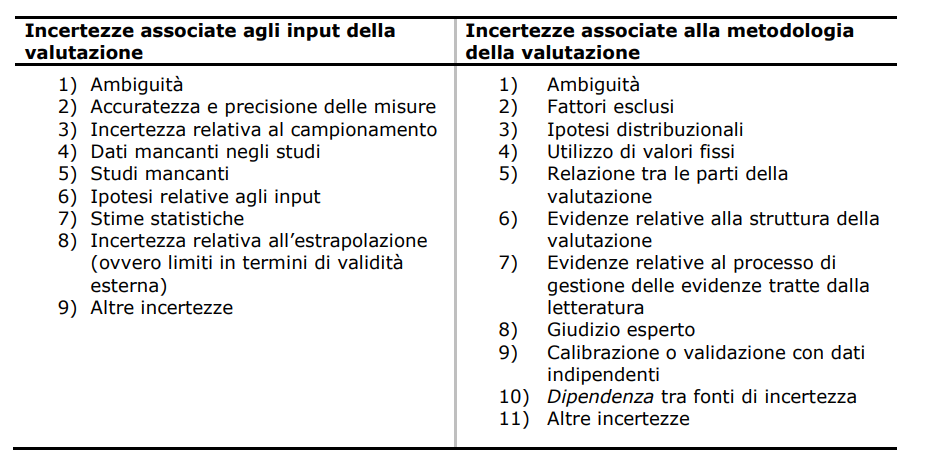
\includegraphics[width=0.9\columnwidth]{tipologia-incertezze} 
    \caption{Natura dell'incertezza}
\end{figure}

\subsubsection{Definizione delle priorità delle incertezze}

Definire le priorità delle fonti di incertezza è utile in diverse fasi della valutazione. All'inizio, aiuta a selezionare le incertezze più importanti per un'analisi approfondita. Durante la valutazione, individua le aree in cui cercare più dati o coinvolgere ulteriori esperti. Alla fine, identifica potenziali aree di ricerca futura. Le priorità dovrebbero basarsi sul contributo di ciascuna fonte di incertezza all'incertezza complessiva della valutazione, tenendo conto della dimensione dell'incertezza e della sua influenza sul risultato.
L'influenza delle diverse incertezze può essere valutata utilizzando giudizi esperti e scale ordinali. Si possono utilizzare metodi come le “tabelle d'incertezza” o l'approccio NUSAP.

Quando si usano modelli quantitativi, l'analisi di sensibilità può valutare l'influenza delle incertezze sugli input del modello. Le scelte riguardanti la struttura del modello possono essere verificate ripetendo la valutazione con alternative.

Per affrontare l'incertezza in modo efficace, è fondamentale che la valutazione sia suddivisa in parti principali, come esposizione e pericoli in una valutazione del rischio chimico, e in parti minori, come singoli parametri o studi. Questa suddivisione consente di eseguire l'analisi dell'incertezza a diversi livelli: valutare tutte le incertezze collettivamente, suddividerle in parti principali e combinarle successivamente, o suddividerle ulteriormente in parti più piccole e combinarle gradualmente. È essenziale combinare le parti dell'analisi per caratterizzare l'incertezza complessiva, definendo in anticipo come queste parti verranno integrate. Utilizzare un diagramma di modello concettuale può migliorare la trasparenza e il rigore del processo.\\

L'efficienza e l'affidabilità della valutazione dipendono dal livello di suddivisione scelto. Trattare separatamente le parti con incertezze rilevanti è generalmente più affidabile, mentre valutare tutte le incertezze collettivamente può essere più rapido ma meno preciso. Alcune incertezze minori possono essere considerate in una fase successiva della caratterizzazione complessiva, mentre quelle maggiori dovrebbero essere combinate tramite calcoli per garantire maggiore affidabilità. Quando si utilizzano modelli quantitativi, è utile quantificare l'incertezza per ciascun parametro e considerare anche le incertezze non quantificate, come quelle relative alla struttura del modello.\\

Per valutare correttamente l'incertezza, è essenziale che le domande e le quantità d'interesse siano chiaramente definite. Qualsiasi ambiguità aggiunge ulteriore incertezza e complica la valutazione. Se una domanda o quantità non è già ben definita, i valutatori devono provvedere a farlo per l'analisi dell'incertezza. Una quantità o domanda è ben definita se i valutatori possono concordare sulla risposta. Per ottenere ciò, si può specificare un esperimento, uno studio o una procedura che determinerebbe la risposta. Ad esempio, una misura ben definita per una quantità d'interesse dovrebbe includere specifiche di tempo, popolazione, luogo e condizioni. Allo stesso modo, la presenza o assenza di condizioni o meccanismi specifici deve essere dettagliata, così come i risultati di uno studio scientifico o un calcolo rilevante per la valutazione. Durante la formulazione delle domande, è importante identificare e sostituire termini ambigui o soggetti a giudizio di gestione del rischio con termini più chiari o numeri. Se i termini di riferimento sono aperti, è necessario che le conclusioni siano riferite a quantità ben definite o contengano affermazioni chiare e ben definite, necessarie per valutare ed esprimere l'incertezza associata.\\

L'espressione qualitativa dell'incertezza utilizza parole o categorie ordinali, senza quantificare le possibili risposte o probabilità. Questo metodo è utile in varie situazioni, come la definizione delle priorità delle incertezze e la descrizione di singole fonti di incertezza durante l'analisi. Le espressioni qualitative sono utili per definire le priorità, descrivere singole fonti di incertezza come passaggio preliminare per la quantificazione complessiva, comunicare i risultati usando una scala di probabilità approssimata con descrittori qualitativi, descrivere incertezze non incluse nella valutazione quantitativa e per la reportistica quando richiesto da decisori o normative.\\

Per descrivere singole fonti di incertezza, si raccomanda l'uso di scale ordinali per migliorare coerenza e trasparenza. Queste scale dovrebbero essere parte della pianificazione della valutazione e possono variare in formalità a seconda delle necessità. Le espressioni qualitative dovrebbero essere usate per elaborare un giudizio quantitativo sull'impatto combinato delle incertezze, basandosi su una logica chiara e non su calcoli arbitrari.\\

\subsection{Quantificare l'incertezza tramite probabilità}

Il Comitato scientifico raccomanda di esprimere quantitativamente l'impatto combinato delle incertezze. Le probabilità, specificate completamente o parzialmente, possono essere derivate da dati o giudizio esperto.\\

\textbf{Probabilità:} La probabilità varia da 0 a 1, espressa come percentuale da 0\% a 100\%. Per una domanda sì/no, 0\% significa che la risposta è sicuramente negativa, 100\% che è sicuramente positiva, e valori intermedi rappresentano vari gradi di certezza.\\

\textbf{Distribuzioni di probabilità:} L'incertezza relativa a una quantità non variabile può essere espressa tramite una distribuzione di probabilità, mostrando la probabilità relativa di diversi valori. Un'espressione parziale dell'incertezza può indicare la probabilità che un intervallo di valori includa il valore reale.\\

\textbf{Uso dei dati:} Quando disponibili, i dati dovrebbero essere utilizzati tramite analisi statistica, anche se il giudizio esperto interviene sempre, ad esempio nella scelta del modello  statistico. L'incertezza può essere quantificata direttamente o tramite calcoli dopo aver quantificato singole fonti di incertezza.\\



\section{Intelligenza artificiale in ambito medico: cosa ne pensano gli utenti nel 2024}

Secondo una recente indagine\footcite{womak:intelligenza-artificiale-e-medicina} dell'EngageMinds HUB, il Centro di ricerca dell'Università Cattolica, gli italiani ad oggi segnalano fiducia e timori verso l'uso dell'intelligenza artificiale in ambito medico.\\
Dal loro studio emerge che 6 italiani su 10 sono favorevoli all'uso dell'Intelligenza artificiale in ambito sanitario, di questi, l'88\% la userebbe per semplificare il linguaggio dei referti, l'86\% come supporto al medico per effettuare una diagnosi e l'80\% come aiuto per stabilire una terapia farmacologica adeguata, mentre quasi 6 italiani su 10 la utilizzerebbero come strumento per un'autoanalisi.\\
Di opinione meno positiva sono 7 italiani su 10 secondo i quali l'AI potrà causare una perdita della relazione e del contatto diretto con il medico.\\

Tra le principali opportunità che l'uso delle tecnologie digitali potranno portare, poco meno di 8 italiani su 10 (78\%) riferiscono che esse porteranno ad una maggiore accessibilità nell'accesso e nell'uso dei servizi, una riduzione dello spreco di carta e un maggior coinvolgimento del paziente grazie ad una maggiore accessibilità al proprio fascicolo sanitario. Il 74\% crede che le AI potranno ridurre i costi a lungo termine; poco meno di 7 su 10 ritengono che possa esserci un miglioramento nei monitoraggi tramite devices (68\%), mentre poco più di 6 su 10 si aspetta che le AI possano migliorare le diagnosi (63\%). Il 68\% degli italiani ritiene che l'uso di tecnologie digitali possano migliorare il monitoraggio da
remoto.\\

Un ulteriore rischio che gli italiani percepiscono è legato ai dati sensibili: per il 63\% l'uso dell'Intelligenza Artificiale potrà causare delle problematiche legate alla gestione della privacy, mentre per il 60\% legate alla diffusione di dati sensibili.


    \backmatter
    \printglossary[type=\acronymtype, title=Acronimi e abbreviazioni, toctitle=Acronimi e abbreviazioni]
    \printglossary[type=main, title=Glossario, toctitle=Glossario]

    \cleardoublepage
\chapter{Bibliografia}

\nocite{*}

% Print book bibliography
\printbibliography[heading=subbibliography,title={Libri di riferimento},type=book]

% Print articles bibliography
\printbibliography[heading=subbibliography,title={Articoli di riferimento},type=article]

% Print site bibliography
\printbibliography[heading=subbibliography,title={Siti web consultati},type=online]

\end{document}
